%%%%%%%%%%%%%%%%%%%%%%%%%%%%%%%%%%%%%%%%%%%%%%%%%%%%%%%%%%%%%%%%%%%%%%
% Overleaf (WriteLaTeX) Example: Molecular Chemistry Presentation
%
% Source: http://www.overleaf.com
%
% In these slides we show how Overleaf can be used with standard 
% chemistry packages to easily create professional presentations.
% 
% Feel free to distribute this example, but please keep the referral
% to overleaf.com
% 
%%%%%%%%%%%%%%%%%%%%%%%%%%%%%%%%%%%%%%%%%%%%%%%%%%%%%%%%%%%%%%%%%%%%%%

\documentclass{beamer}

\mode<presentation>
{
  \usetheme{Madrid}       % or try default, Darmstadt, Warsaw, ...
  \usecolortheme{default} % or try albatross, beaver, crane, ...
  \usefonttheme{default}    % or try default, structurebold, ...
  \setbeamertemplate{navigation symbols}{}
  \setbeamertemplate{caption}[numbered]
} 

\usepackage[english]{babel}
\usepackage[utf8x]{inputenc}
\usepackage{graphicx}
\usepackage{hyperref}
  \hypersetup{colorlinks=true}
  \hypersetup{urlcolor=blue}
  \hypersetup{linkcolor = .}
\usepackage{xcolor}
\usepackage{siunitx}
  \sisetup{separate-uncertainty = true}
\usepackage{physics}
\usepackage[font=small,labelfont=bf,justification=centering]{caption}
\usepackage{subcaption}
\usepackage[en-GB]{datetime2}
\usepackage{overpic}
\usepackage{feynmp}
\DeclareGraphicsRule{*}{mps}{*}{}
\usepackage{scalerel}
\newcommand{\mylbrace}[2]{\vspace{#2pt}\hspace{6pt}\scaleleftright[\dimexpr5pt+#1\dimexpr0.06pt]{\lbrace}{\rule[\dimexpr2pt-#1\dimexpr0.5pt]{-4pt}{#1pt}}{.}}
\newcommand{\myrbrace}[2]{\vspace{#2pt}\scaleleftright[\dimexpr5pt+#1\dimexpr0.06pt]{.}{\rule[\dimexpr2pt-#1\dimexpr0.5pt]{-4pt}{#1pt}}{\rbrace}\hspace{6pt}}
\usepackage{ulem} % Line across text

% Here's where the presentation starts, with the info for the title slide
\title[$K^+K^-\pi^+\pi^-$]{\texorpdfstring{$D\to K^+K^-\pi^+\pi^-$}{K+K-pi+pi-} strong phase analysis at BESIII}

\author{Martin Tat}
\institute{Oxford LHCb}
\date{27th February 2023}

\titlegraphic{
\includegraphics[height = 2cm]{lhcb.jpg}\hspace{1cm}~%
              
\includegraphics[height = 2cm]{OxfordLogo.pdf}\hspace{1cm}~%
              
\includegraphics[height = 2cm]{bes3.jpg}}

\begin{document}

\begin{frame}
  \titlepage
\end{frame}

% These three lines create an automatically generated table of contents.
%\begin{frame}{Outline}
%  \tableofcontents
%\end{frame}

\section{Recap of BESIII analysis}
\begin{frame}{Recap of BESIII analysis}
  \begin{center}
    {\huge Recap of BESIII analysis}
  \end{center}
\end{frame}

\begin{frame}{Recap of BESIII analysis}
  \begin{center}
    \Large{Analysis of $D^0\to K^+K^-\pi^+\pi^-$}
  \end{center}
  \vspace{0.5cm}
  \begin{itemize}
    \setlength\itemsep{1.0em}
    \item{Study $D^0$-$\bar{D^0}$ strong phase difference in bins of the 5D phase space}
    \item{Measurement of amplitude averaged strong phases $c_i$ and $s_i$}
    \item{$c_i$ and $s_i$ are important inputs to the $\gamma$ measurement at LHCb}
    \begin{itemize}
      \item{LHCb result: $\gamma = (116^{+12}_{-14})^\circ$ with model dependent inputs}
      \item{$\gamma$ may change when updated with model independent $c_i$ and $s_i$}
    \end{itemize}
    \item{Measurement technique unique to charm factories: Study decays of quantum correlated $D\bar{D}$ pairs using a double tag method}
  \end{itemize}
\end{frame}

\begin{frame}{Recap of BESIII analysis}
  \begin{itemize}
    \item{$\psi(3770)\to D^0\bar{D^0}$ decay conserves $\mathcal{C} = -1$}
  \end{itemize}
  \begin{figure}[H]
    \centering
    \vspace{-1.5cm}
    \begin{fmffile}{fgraph/fgraph_ee1}
      \setlength{\unitlength}{1cm}
      \begin{fmfgraph*}(8,5)
        \fmfleft{i}
        \fmfright{o}
        \fmflabel{$D^0$}{i}
        \fmflabel{$\bar{D^0}$}{o}
        \fmf{fermion}{w,i}
        \fmf{fermion}{w,o}
        \fmfblob{1cm}{w}
        \fmfv{label=$\psi(3770)$,label.dist=15,label.angle=90}{w}
      \end{fmfgraph*}
    \end{fmffile}
    \vspace{-2.0cm}
  \end{figure}
  \begin{itemize}
    \item{But since they are quantum correlated, we must consider their CP eigenstates $D_\pm = (\lvert D^0\rangle\pm\lvert\bar{D^0}\rangle)/\sqrt{2}$}
    \item{Total wavefunction is $\lvert D^0\rangle\lvert\bar{D^0}\rangle - \lvert\bar{D^0}\rangle\lvert D^0\rangle = \lvert D_+\rangle\lvert D_-\rangle + \lvert D_-\rangle\lvert D_+\rangle$}
  \end{itemize}
  \begin{figure}[H]
    \centering
    \vspace{-1.5cm}
    \begin{fmffile}{fgraph/fgraph_ee2}
      \setlength{\unitlength}{1cm}
      \begin{fmfgraph*}(8,5)
        \fmfleft{i}
        \fmfright{o}
        \fmflabel{$D_+$}{i}
        \fmflabel{$D_-$}{o}
        \fmf{fermion}{w,i}
        \fmf{fermion}{w,o}
        \fmfblob{1cm}{w}
        \fmfv{label=$\psi(3770)$,label.dist=15,label.angle=90}{w}
      \end{fmfgraph*}
    \end{fmffile}
    \vspace{-2.0cm}
  \end{figure}
  \begin{center}
    The two $D$ mesons do \underline{not} communicate, but the $D\to KK\pi\pi$ decay is perfectly correlated with the tagged $D$
  \end{center}
\end{frame}

\begin{frame}{Recap of BESIII analysis}
  \begin{itemize}
    \item{Tag mode can be a \underline{flavour tag}}
    \begin{itemize}
      \item{$K\pi$, $K\pi\pi^0$, $K\pi\pi\pi$, $Ke\nu$}
    \end{itemize}
  \end{itemize}
  \begin{figure}[H]
    \centering
    \vspace{0.3cm}
    \begin{fmffile}{fgraph/fgraph_flavour_tag}
      \setlength{\unitlength}{1cm}
      \begin{fmfgraph*}(8,4)
        \fmfstraight
        \fmfleft{i4,i3,i2,i1}
        \fmfright{g1,o1,o2,g2}
        \fmflabel{$\pi^+$}{o1}
        \fmflabel{$K^-$}{o2}
        \fmflabel{$K^+$}{i1}
        \fmflabel{$K^-$}{i2}
        \fmflabel{$\pi^+$}{i3}
        \fmflabel{$\pi^-$}{i4}
        \fmf{fermion}{w,i1}
        \fmf{fermion}{w,i2}
        \fmf{fermion}{w,i3}
        \fmf{fermion}{w,i4}
        \fmf{fermion}{w,o1}
        \fmf{fermion}{w,o2}
        \fmf{phantom}{w,g1}
        \fmf{phantom}{w,g2}
        \fmfblob{1cm}{w}
      \end{fmfgraph*}
    \end{fmffile}
    \vspace{0.3cm}
  \end{figure}
  \begin{center}
    Use flavour tags to measure fraction of $D^0\to KK\pi\pi$ decays in bin $i$:\\
    $\frac{N^{\rm DT}_i}{N^{\rm ST}} = \mathcal{B}(KK\pi\pi)\times K_i$
  \end{center}
\end{frame}

\begin{frame}{Recap of BESIII analysis}
  \begin{itemize}
    \item{Tag mode can be a \underline{CP even tag}}
    \begin{itemize}
      \item{$KK$, $\pi\pi$, $\pi\pi\pi^0$, $K_S\pi^0\pi^0$, $K_L\pi^0$, $K_L\omega$}
    \end{itemize}
  \end{itemize}
  \begin{figure}[H]
    \centering
    \vspace{0.3cm}
    \begin{fmffile}{fgraph/fgraph_CPeven_tag}
      \setlength{\unitlength}{1cm}
      \begin{fmfgraph*}(8,4)
        \fmfstraight
        \fmfleft{i4,i3,i2,i1}
        \fmfright{g1,o1,o2,g2}
        \fmflabel{$K^+$}{o1}
        \fmflabel{$K^-$}{o2}
        \fmflabel{$K^+$}{i1}
        \fmflabel{$K^-$}{i2}
        \fmflabel{$\pi^+$}{i3}
        \fmflabel{$\pi^-$}{i4}
        \fmf{fermion}{w,i1}
        \fmf{fermion}{w,i2}
        \fmf{fermion}{w,i3}
        \fmf{fermion}{w,i4}
        \fmf{fermion}{w,o1}
        \fmf{fermion}{w,o2}
        \fmf{phantom}{w,g1}
        \fmf{phantom}{w,g2}
        \fmfblob{1cm}{w}
      \end{fmfgraph*}
    \end{fmffile}
    \vspace{0.3cm}
  \end{figure}
  \begin{center}
    $D\to K^+K^-$, which is $C\!P$ even, forces $D\to K^+K^-\pi^+\pi^-$ to be $C\!P$ odd
  \end{center}
\end{frame}

\begin{frame}{Recap of BESIII analysis}
  \begin{itemize}
    \item{Tag mode can be a \underline{CP odd tag}}
    \begin{itemize}
      \item{$K_S\pi^0$, $K_S\omega$, $K_S\eta$, $K_S\eta'$, $K_L\pi^0\pi^0$}
    \end{itemize}
  \end{itemize}
  \begin{figure}[H]
    \centering
    \vspace{0.3cm}
    \begin{fmffile}{fgraph/fgraph_CPodd_tag}
      \setlength{\unitlength}{1cm}
      \begin{fmfgraph*}(8,4)
        \fmfstraight
        \fmfleft{i4,i3,i2,i1}
        \fmfright{g1,o1,o2,g2}
        \fmflabel{$\pi^0$}{o1}
        \fmflabel{$K_S$}{o2}
        \fmflabel{$K^+$}{i1}
        \fmflabel{$K^-$}{i2}
        \fmflabel{$\pi^+$}{i3}
        \fmflabel{$\pi^-$}{i4}
        \fmf{fermion}{w,i1}
        \fmf{fermion}{w,i2}
        \fmf{fermion}{w,i3}
        \fmf{fermion}{w,i4}
        \fmf{fermion}{w,o1}
        \fmf{fermion}{w,o2}
        \fmf{phantom}{w,g1}
        \fmf{phantom}{w,g2}
        \fmfblob{1cm}{w}
      \end{fmfgraph*}
    \end{fmffile}
    \vspace{0.3cm}
  \end{figure}
  \begin{center}
    $D\to K_S^0\pi^0$, which is $C\!P$ odd, forces $D\to K^+K^-\pi^+\pi^-$ to be $C\!P$ even
  \end{center}
\end{frame}

\begin{frame}{Recap of BESIII analysis}
  \begin{center}
    The asymmetry between CP even and CP odd double tag yields is sensitive to $c_i$:\\
    $\frac{N^{\rm DT}_i}{N^{\rm ST}} = \mathcal{B}(KK\pi\pi)\times(K_i + \bar{K_i} \pm 2\sqrt{K_i\bar{K_i}}c_i)$
  \end{center}
  \begin{columns}[onlytextwidth]
    \begin{column}{0.6\textwidth}
      \centering
      \begin{enumerate}
        \setlength\itemsep{1.0em}
        \item{$K_i$: Fraction of $D^0$ decays in bin $i$}
        \item{$\bar{K_i}$: Fraction of $\bar{D^0}$ decays in bin $i$}
        \item{$2\sqrt{K_i\bar{K_i}}c_i$: Interference term, which depend on the cosine of the phase difference between $D^0$ and $\bar{D^0}$ decays}
      \end{enumerate}
    \end{column}
    \begin{column}{0.4\textwidth}
      \begin{figure}
        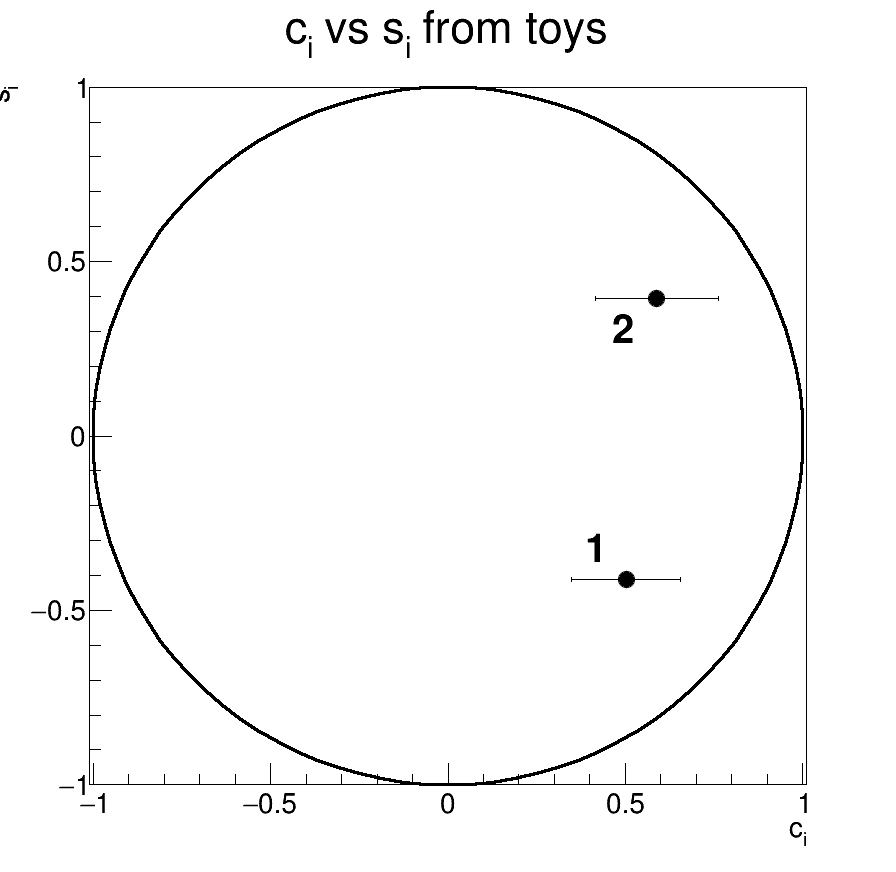
\includegraphics[width = 1.0\textwidth]{Plots/cisi_toys.png}
      \end{figure}
    \end{column}
  \end{columns}
\end{frame}

\section{Double tag yields of partially reconstructed events}
\begin{frame}{Double tag yields of partially reconstructed events}
  \begin{center}
    {\huge Double tag yields of partially reconstructed events}
  \end{center}
\end{frame}

\begin{frame}{Double tag yields of partially reconstructed events}
  \begin{itemize}
    \item{Reconstruction efficiency of $D\to KK\pi\pi$ is very low ($18\%$), compared to other four body modes such as $D\to\pi\pi\pi\pi$ ($49\%$)}
    \begin{itemize}
      \item{Soft kaons get stuck in magnetic field...}
    \end{itemize}
    \item{Try out partially reconstructed $D\to KK\pi\pi$ technique}
    \begin{itemize}
      \item{\underline{No} overlap with the fully reconstructed sample}
    \end{itemize}
  \end{itemize}
  \begin{figure}[H]
    \centering
    \vspace{0.3cm}
    \begin{fmffile}{fgraph/fgraph_CPeven_tag_PartReco}
      \setlength{\unitlength}{1cm}
      \begin{fmfgraph*}(8,4)
        \fmfstraight
        \fmfleft{i4,i3,i2,i1}
        \fmfright{g1,o1,o2,g2}
        \fmflabel{$K^+$}{o1}
        \fmflabel{$K^-$}{o2}
        \fmflabel{$K^+$}{i1}
        \fmflabel{$K^-$}{i2}
        \fmflabel{$\pi^+$}{i3}
        \fmflabel{$\pi^-$}{i4}
        \fmf{dashes}{w,i1}
        \fmf{fermion}{w,i2}
        \fmf{fermion}{w,i3}
        \fmf{fermion}{w,i4}
        \fmf{fermion}{w,o1}
        \fmf{fermion}{w,o2}
        \fmf{phantom}{w,g1}
        \fmf{phantom}{w,g2}
        \fmfblob{1cm}{w}
      \end{fmfgraph*}
    \end{fmffile}
    \vspace{0.3cm}
  \end{figure}
  \begin{center}
    In MC, the yields were found to be similar to fully reconstructed DTs
  \end{center}
\end{frame}

\begin{frame}{Double tag yields of partially reconstructed events}
  \begin{center}
    First look at partially reconstructed $D\to KK\pi\pi$ vs $D\to KK$:
  \end{center}
  \vspace{-0.2cm}
  \begin{figure}
    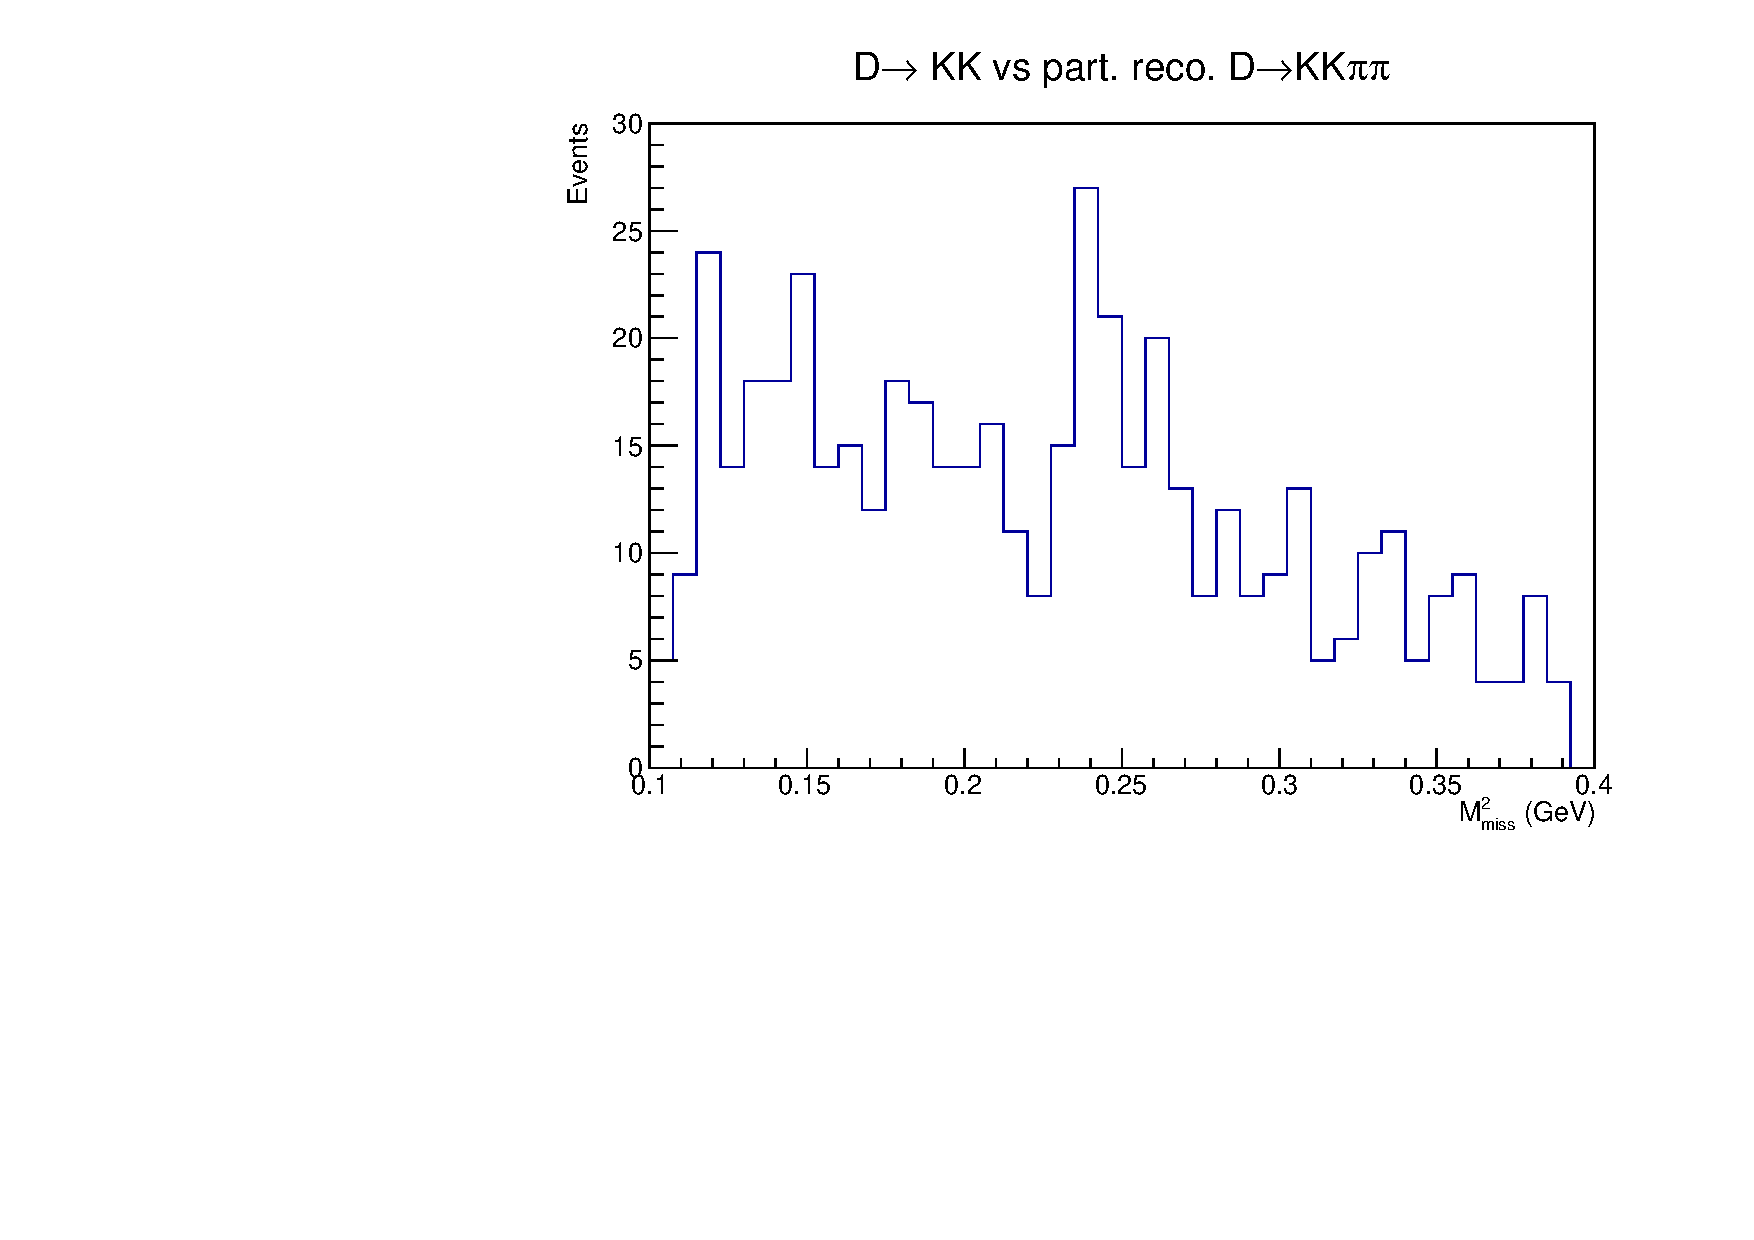
\includegraphics[width = 0.5\textwidth]{Plots/KKPartReco_Mmiss2_NoCuts.pdf}
  \end{figure}
  \vspace{-0.3cm}
  \begin{itemize}
    \setlength\itemsep{0.5em}
    \item{Large background from $D\to K\pi\pi\pi\pi^0$, $\pi\pi^0$ not reconstructed}
    \item{Background is non-peaking since two particles are missing}
    \item{No reliable MC because no model for this decay exists!}
  \end{itemize}
\end{frame}

\begin{frame}{Double tag yields of partially reconstructed events}
  \begin{center}
    Method for removing $\pi^0$ backgrounds: Veto events with $\pi^0$ candidates\\
    Signal efficiency is reduced by $30\%$, but $65\%$ of $K\pi\pi\pi\pi^0$ is rejected
  \end{center}
  \vspace{-0.2cm}
  \begin{figure}
    \centering
    \begin{subfigure}{0.32\textwidth}
      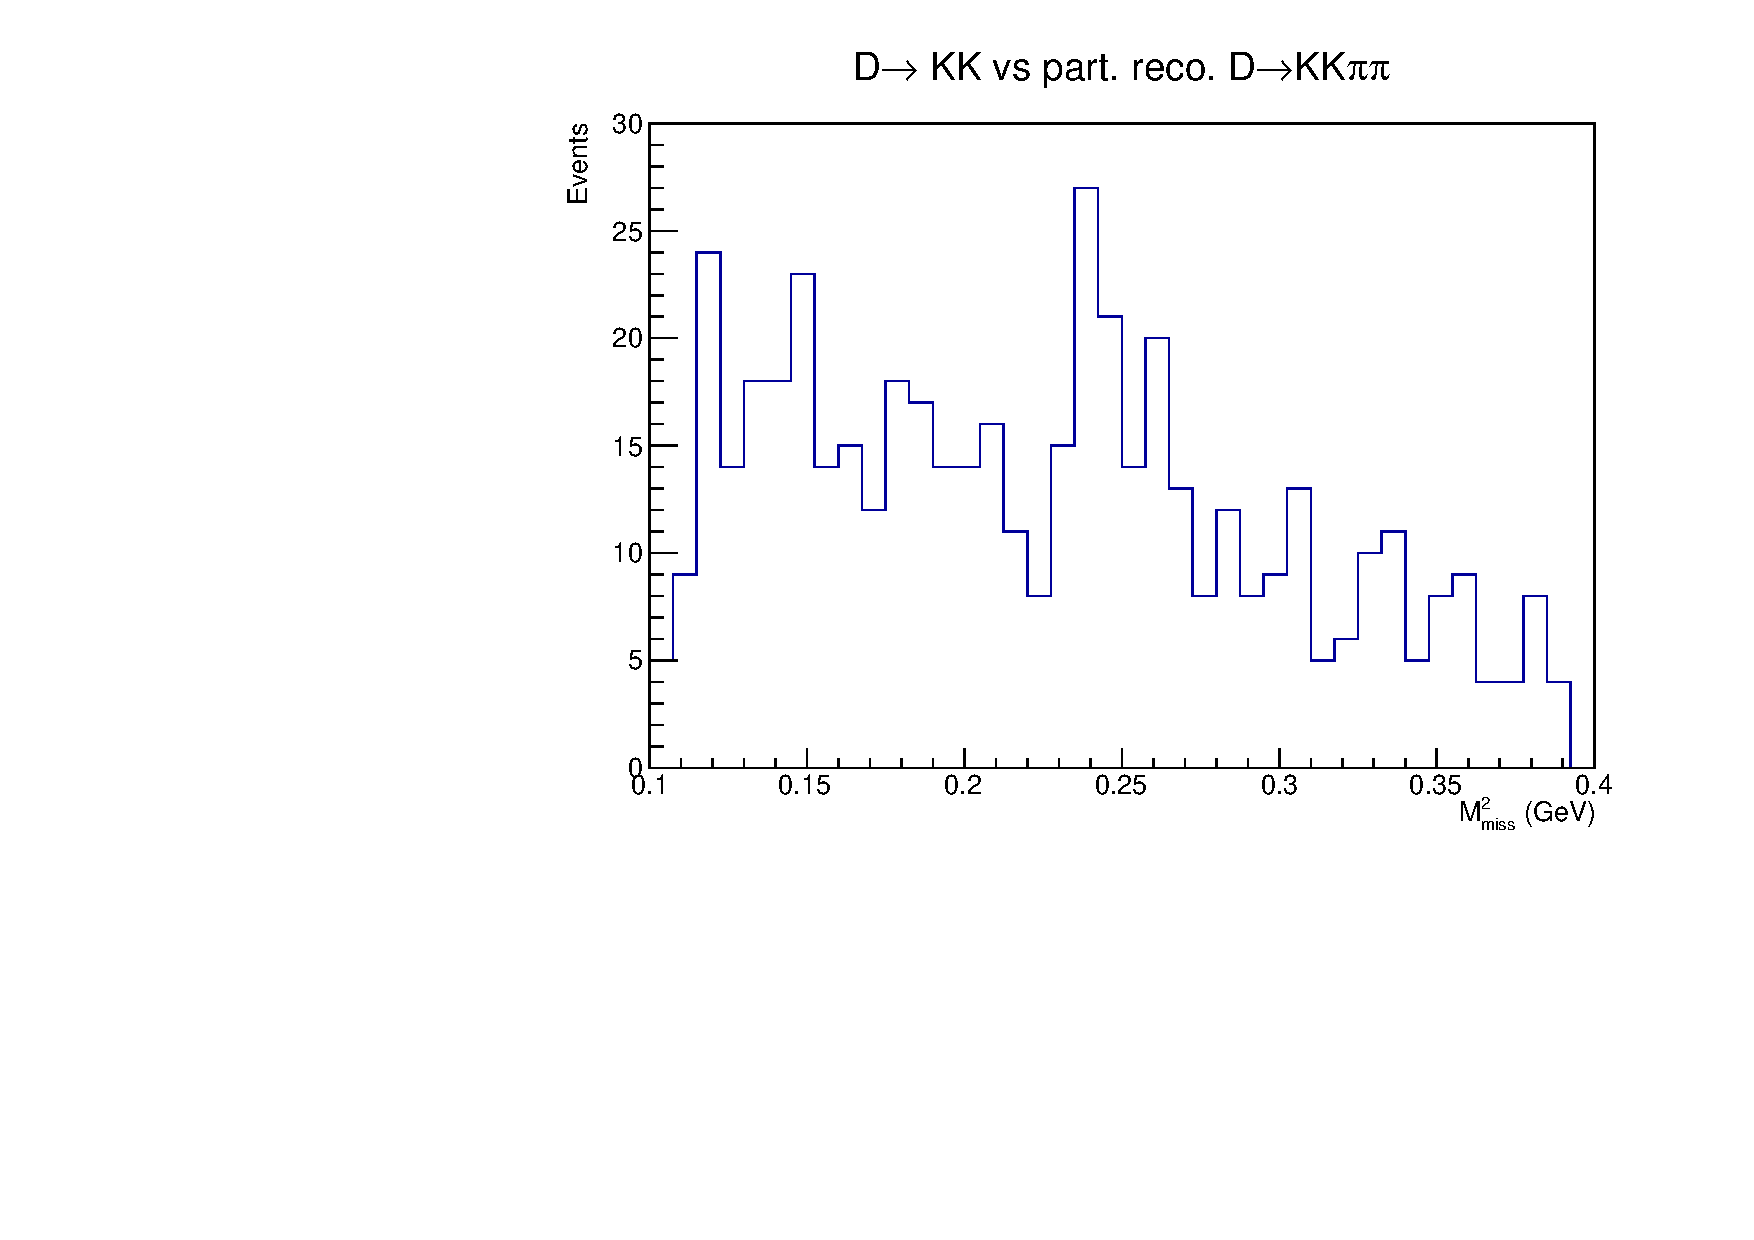
\includegraphics[width = 1.0\textwidth]{Plots/KKPartReco_Mmiss2_NoCuts.pdf}
      \caption{Data, without veto}
    \end{subfigure}%
    \begin{subfigure}{0.32\textwidth}
      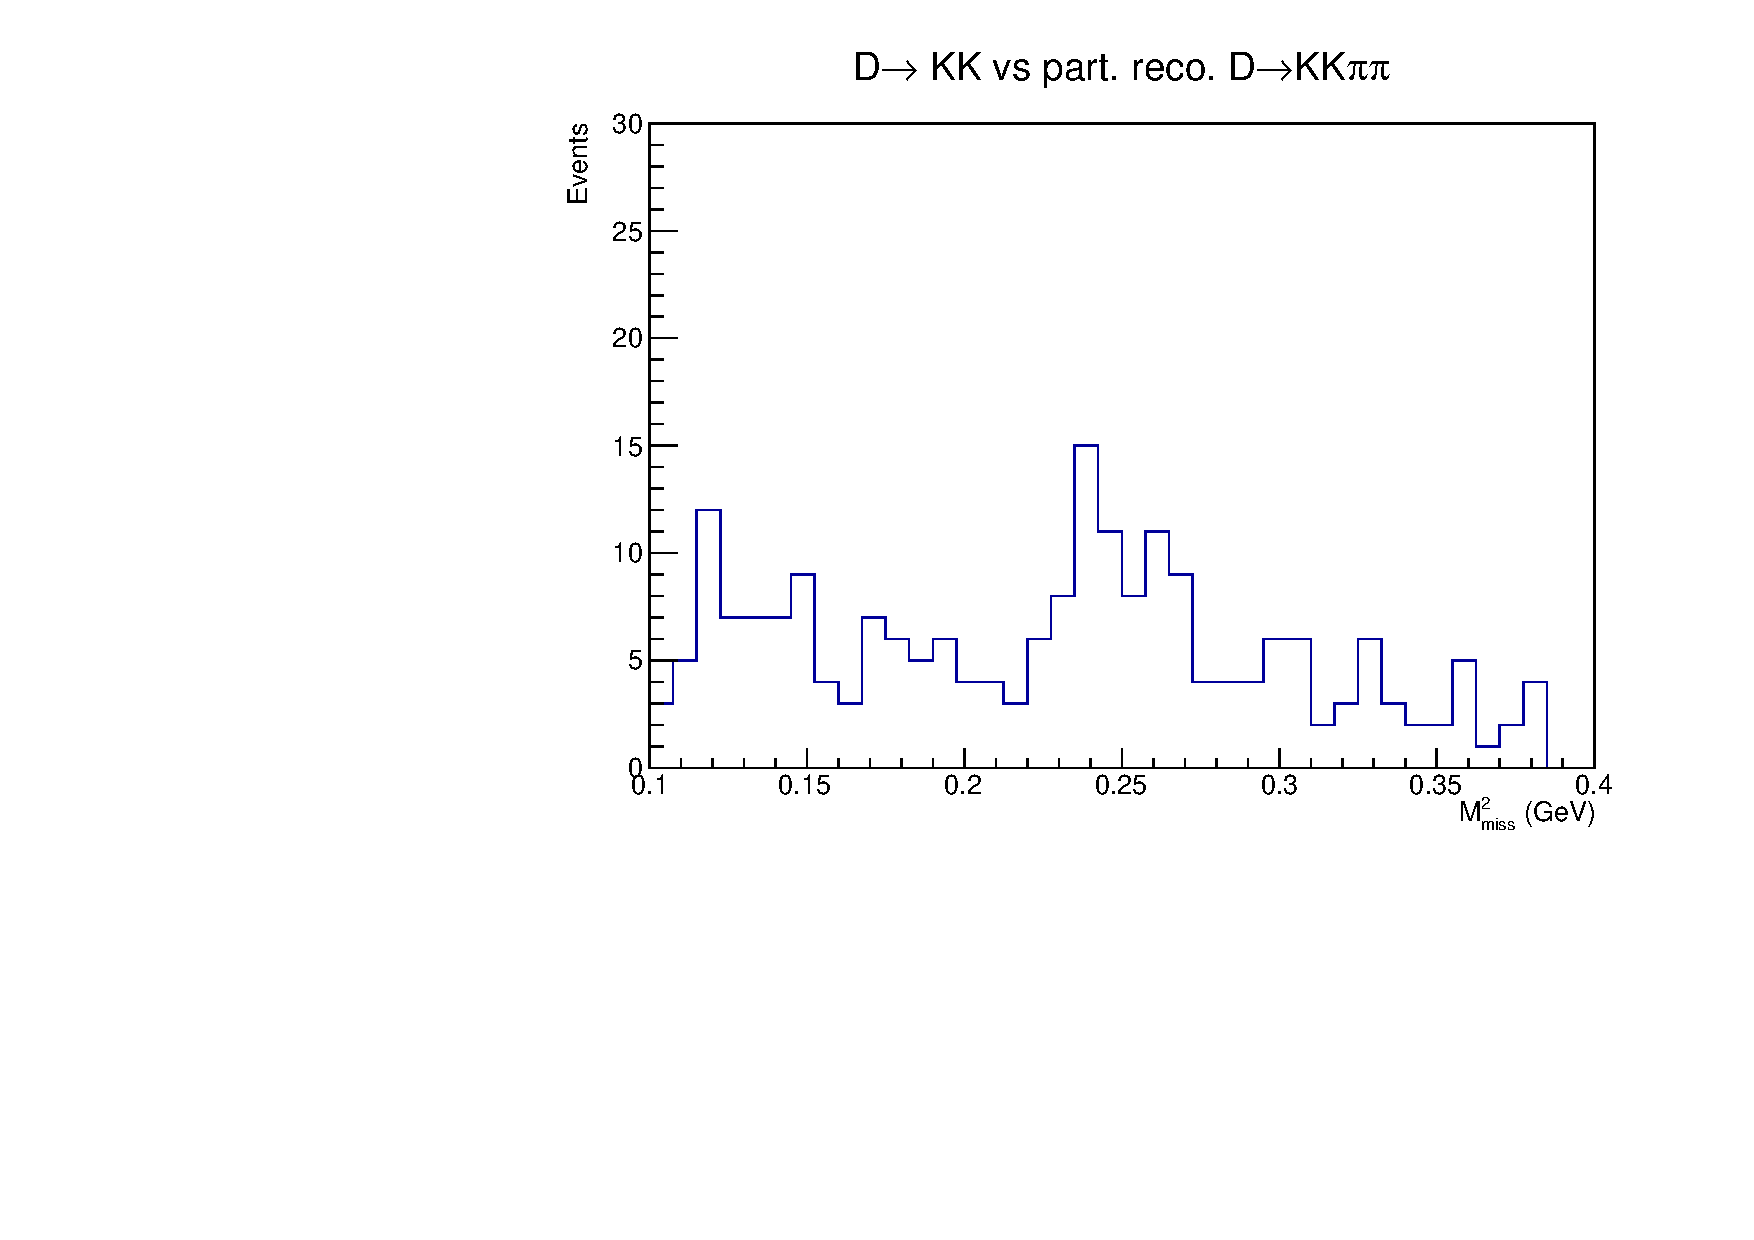
\includegraphics[width = 1.0\textwidth]{Plots/KKPartReco_Mmiss2_Pi0Veto.pdf}
      \caption{Data, with $\pi^0$ veto}
    \end{subfigure}%
    \begin{subfigure}{0.32\textwidth}
      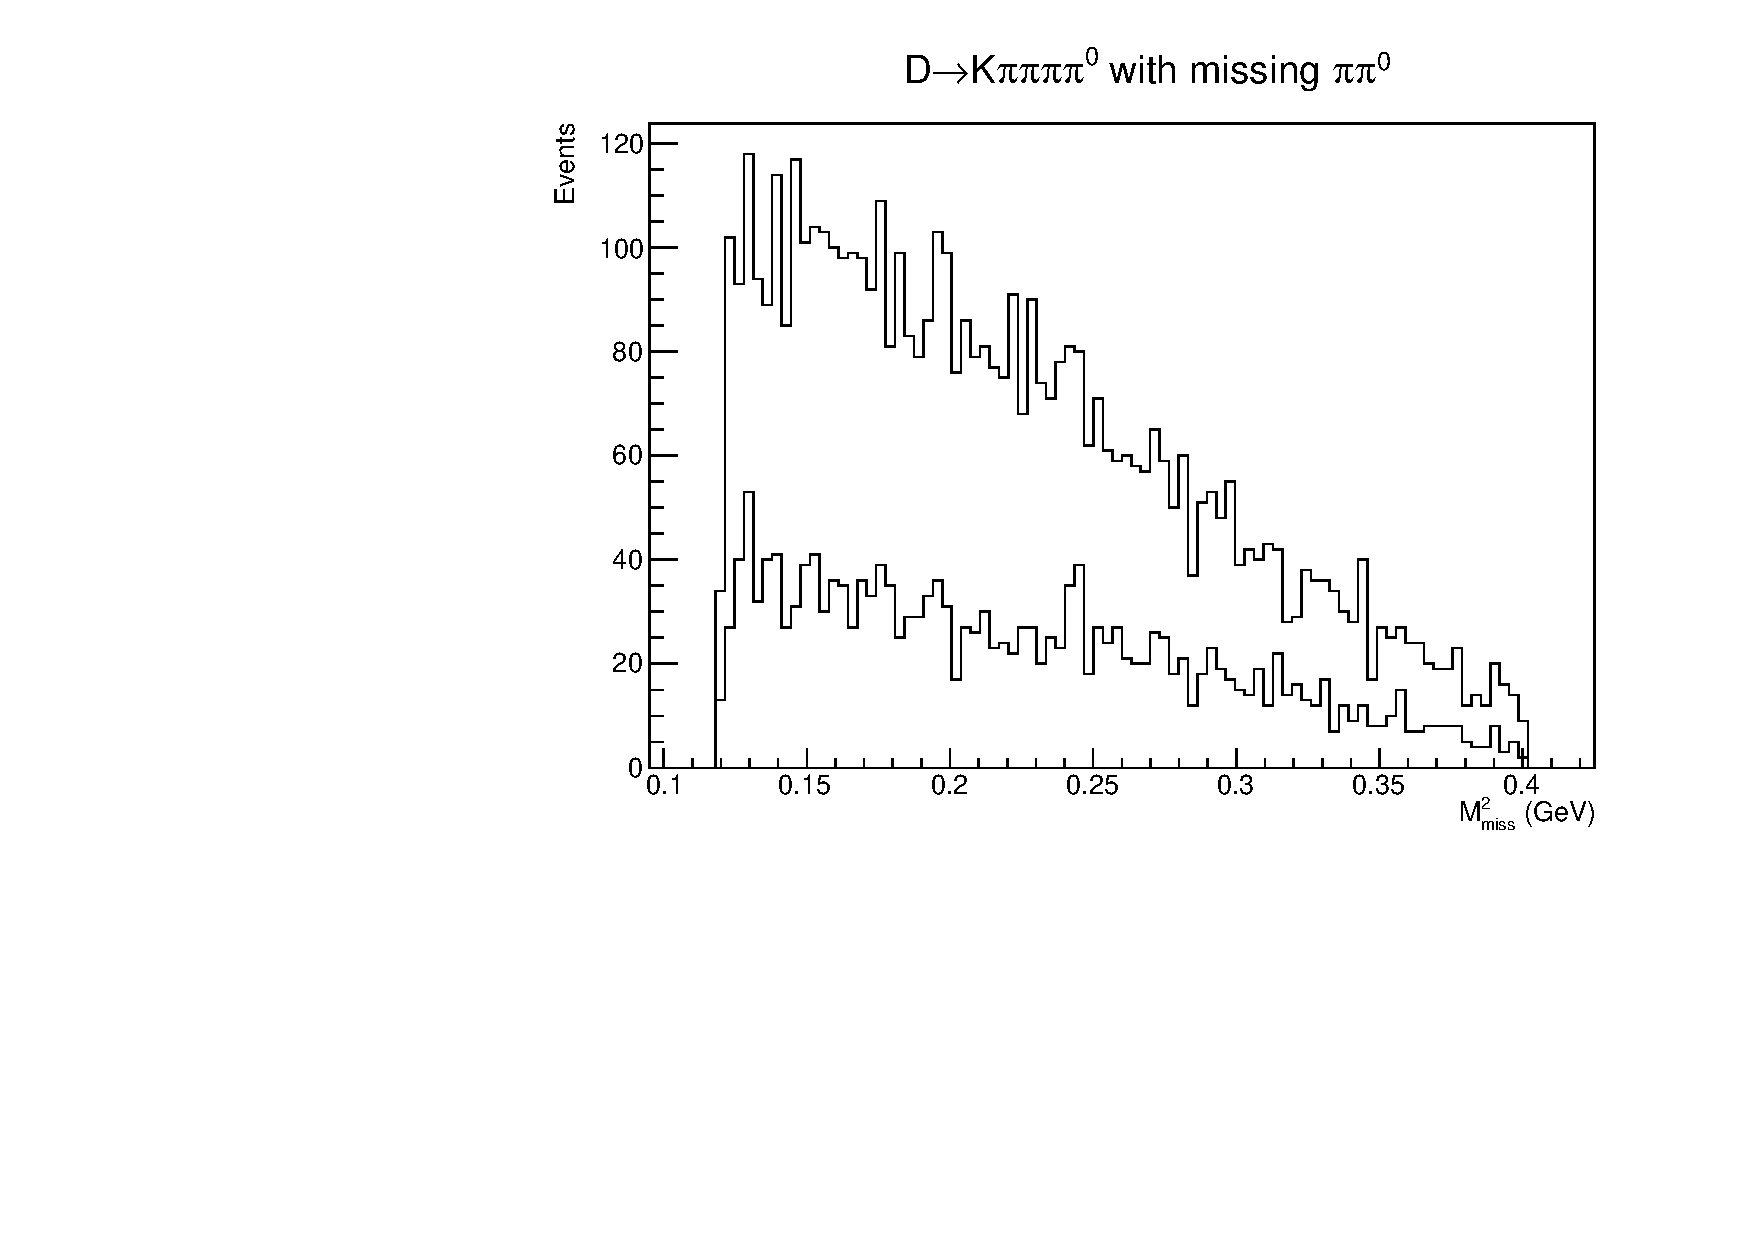
\includegraphics[width = 1.0\textwidth]{Plots/Kpipipipi0_Pi0Veto.pdf}
      \caption{MC, with/without veto}
    \end{subfigure}
    \caption{Study of $\pi^0$ veto}
  \end{figure}
\end{frame}

\begin{frame}{Double tag yields of partially reconstructed events}
  \begin{center}
    Using the method of trial and error, I also discovered that a cut on the kaon energy is highly efficient at removing the $K\pi\pi\pi\pi^0$ background:
  \end{center}
  \vspace{-0.2cm}
  \begin{figure}
    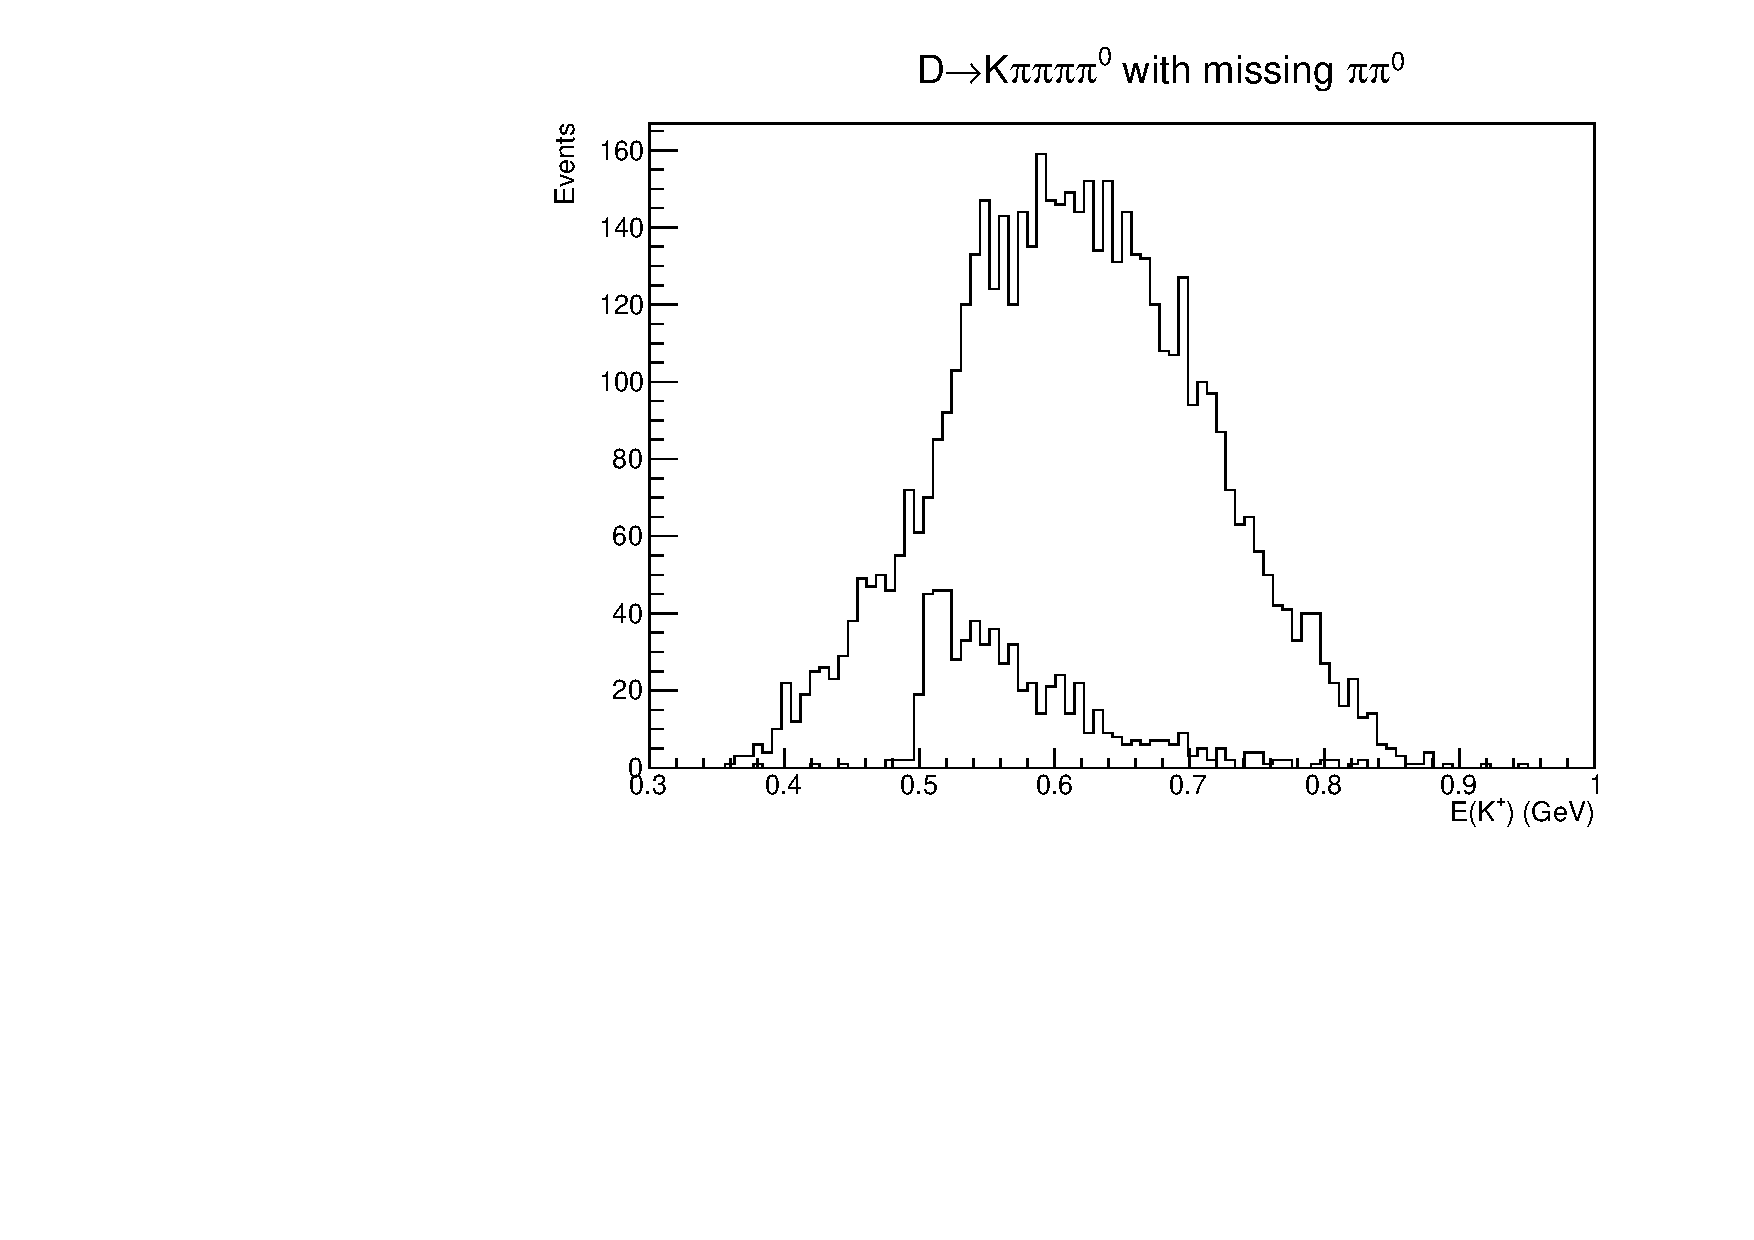
\includegraphics[width = 0.7\textwidth]{Plots/Kpipipipi0_KaonEnergyCut.pdf}
    \caption{The energy spectrum of the kaon from the background $D\to K\pi\pi\pi\pi^0$ and the signal $D\to KK\pi\pi$}
  \end{figure}
\end{frame}

\begin{frame}{Double tag yields of partially reconstructed events}
  \begin{center}
    Unfortunately a cut of $E > m_K$ affects the mass shape...
  \end{center}
  \vspace{-0.2cm}
  \begin{figure}
    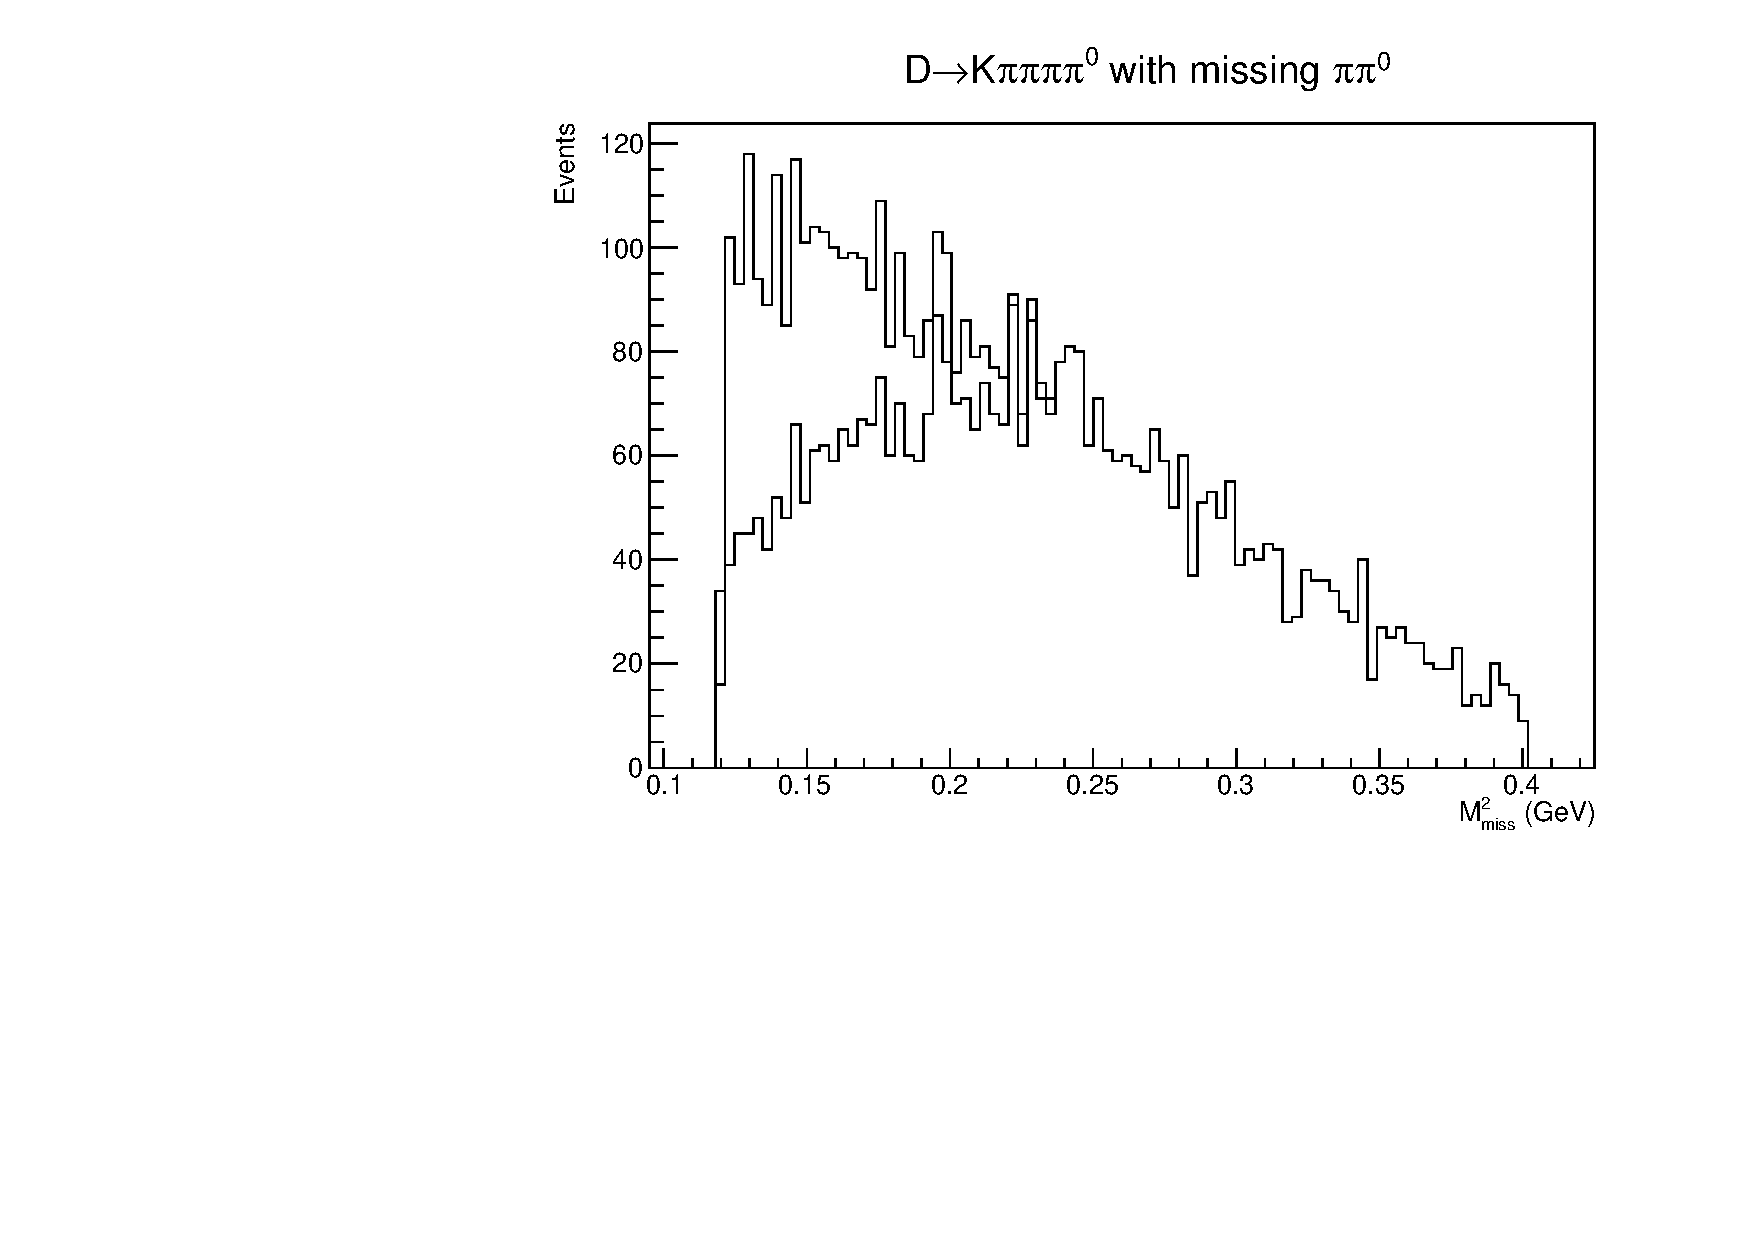
\includegraphics[width = 0.7\textwidth]{Plots/Kpipipipi0_KaonEnergyLowerCut.pdf}
    \caption{Mass shape before and after a $E > m_K$ cut}
  \end{figure}
\end{frame}

\begin{frame}{Double tag yields of partially reconstructed events}
  \begin{center}
    ... but luckily a $E < \SI{0.7}{\giga\eV}$ cut does not change the mass shape!
  \end{center}
  \vspace{-0.2cm}
  \begin{figure}
    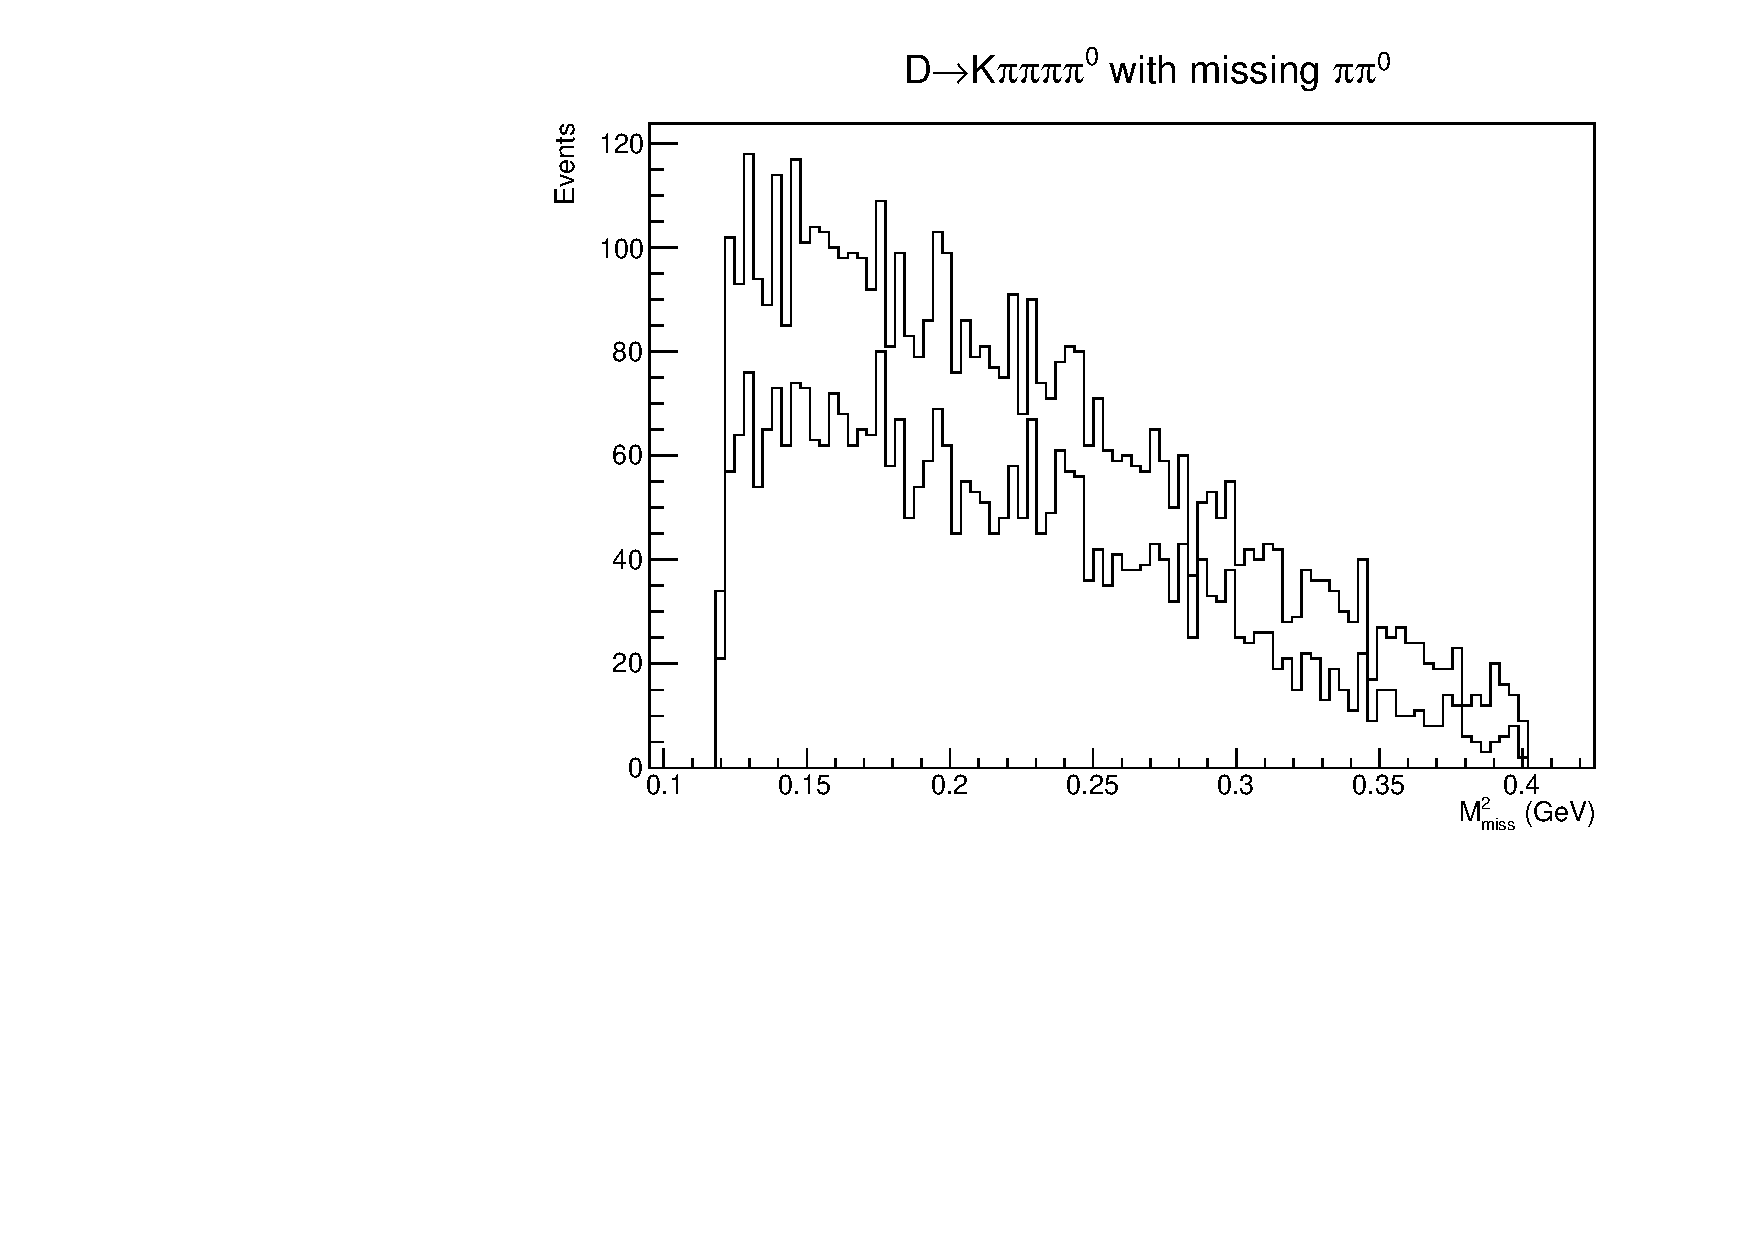
\includegraphics[width = 0.7\textwidth]{Plots/Kpipipipi0_KaonEnergyUpperCut.pdf}
    \caption{Mass shape before and after a $E < \SI{0.7}{\giga\eV}$ cut}
  \end{figure}
\end{frame}

\begin{frame}{Double tag yields of partially reconstructed events}
  \begin{center}
    Finally, I can run the fit and the yields were found to be similar to the fully reconstructed samples
  \end{center}
  \begin{figure}
    \centering
    \begin{subfigure}{0.4\textwidth}
      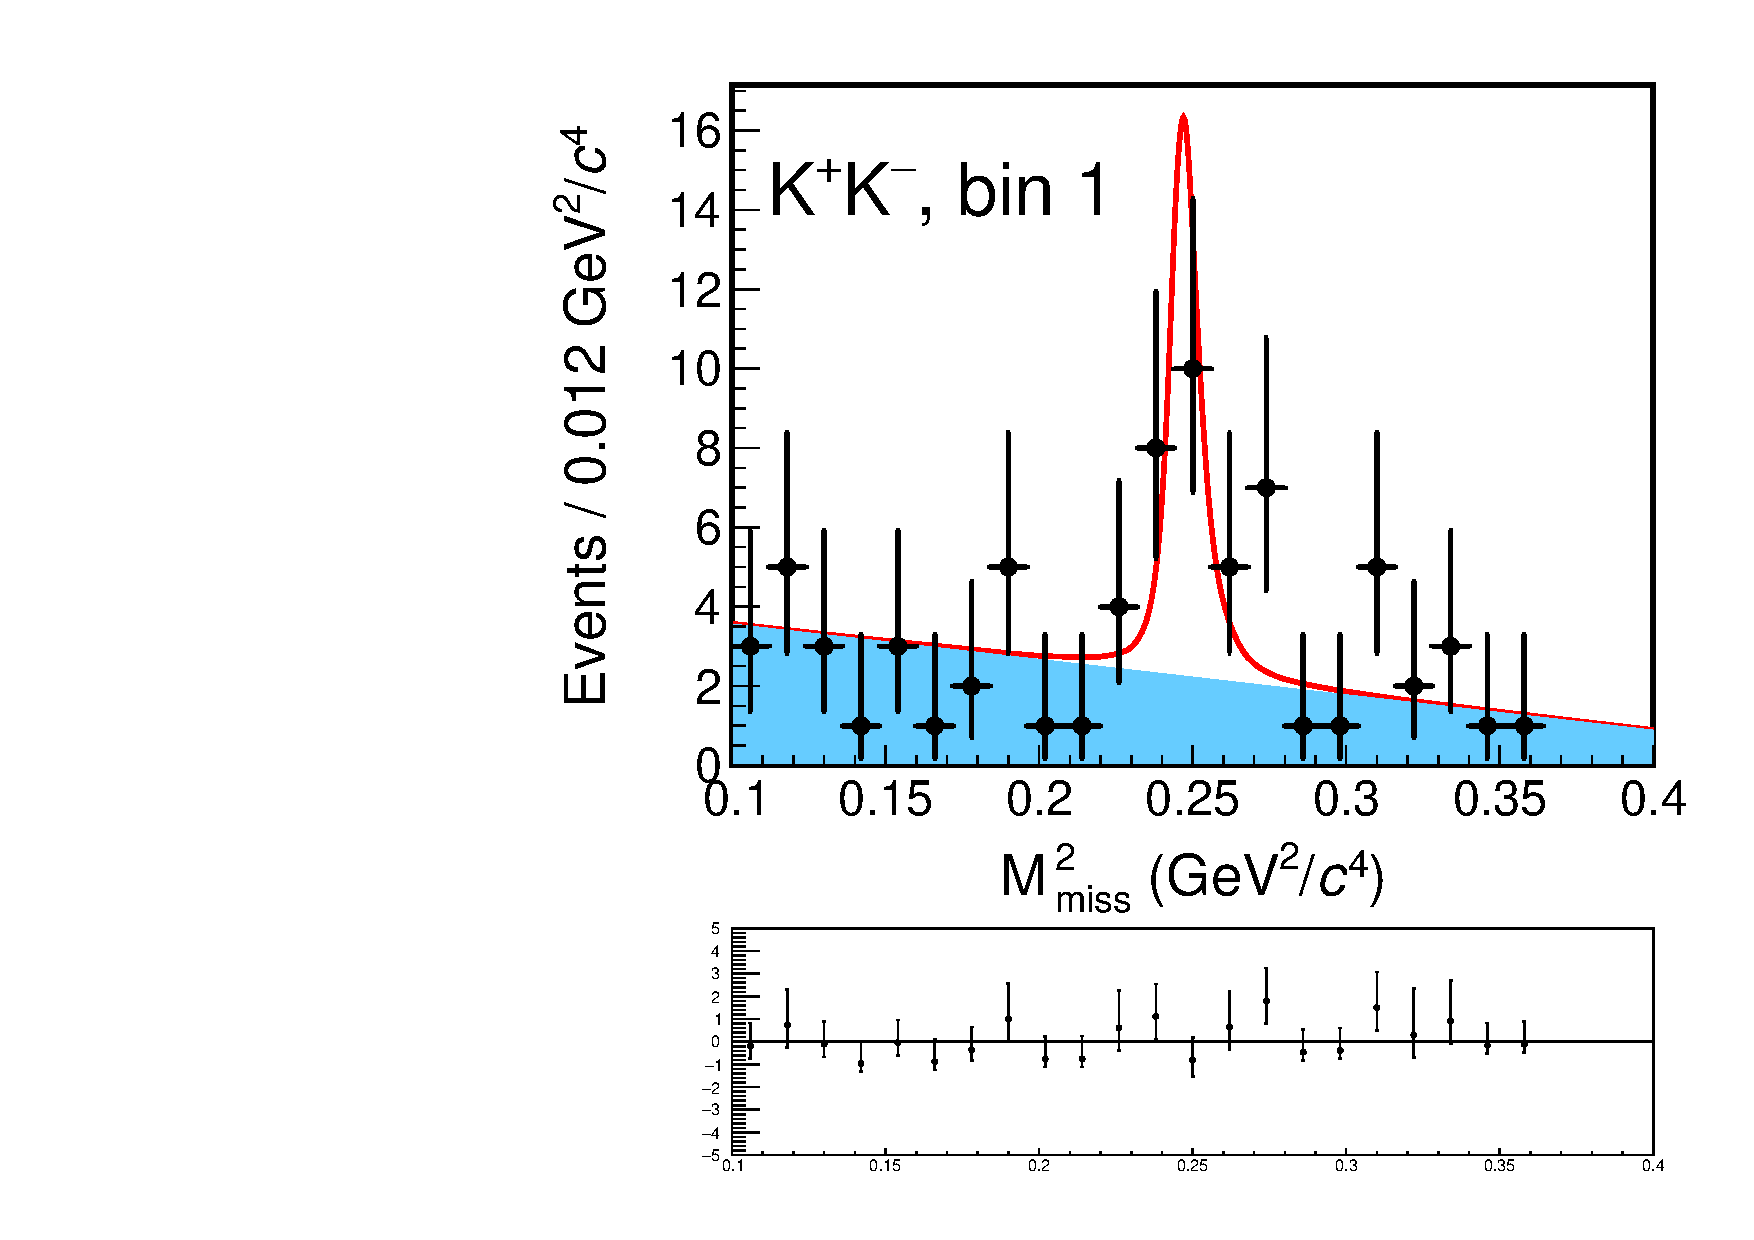
\includegraphics[width = 1.0\textwidth,trim={0 5cm 0 0},clip=true]{Plots/DoubleTagYield_DoubleTag_CP_KKpipi_vs_KKPartReco_SignalBin1.pdf}
      \caption{Bin 1, $N^{\rm DT} = 17.3^{+5.9}_{-5.0}$}
    \end{subfigure}%
    \begin{subfigure}{0.4\textwidth}
      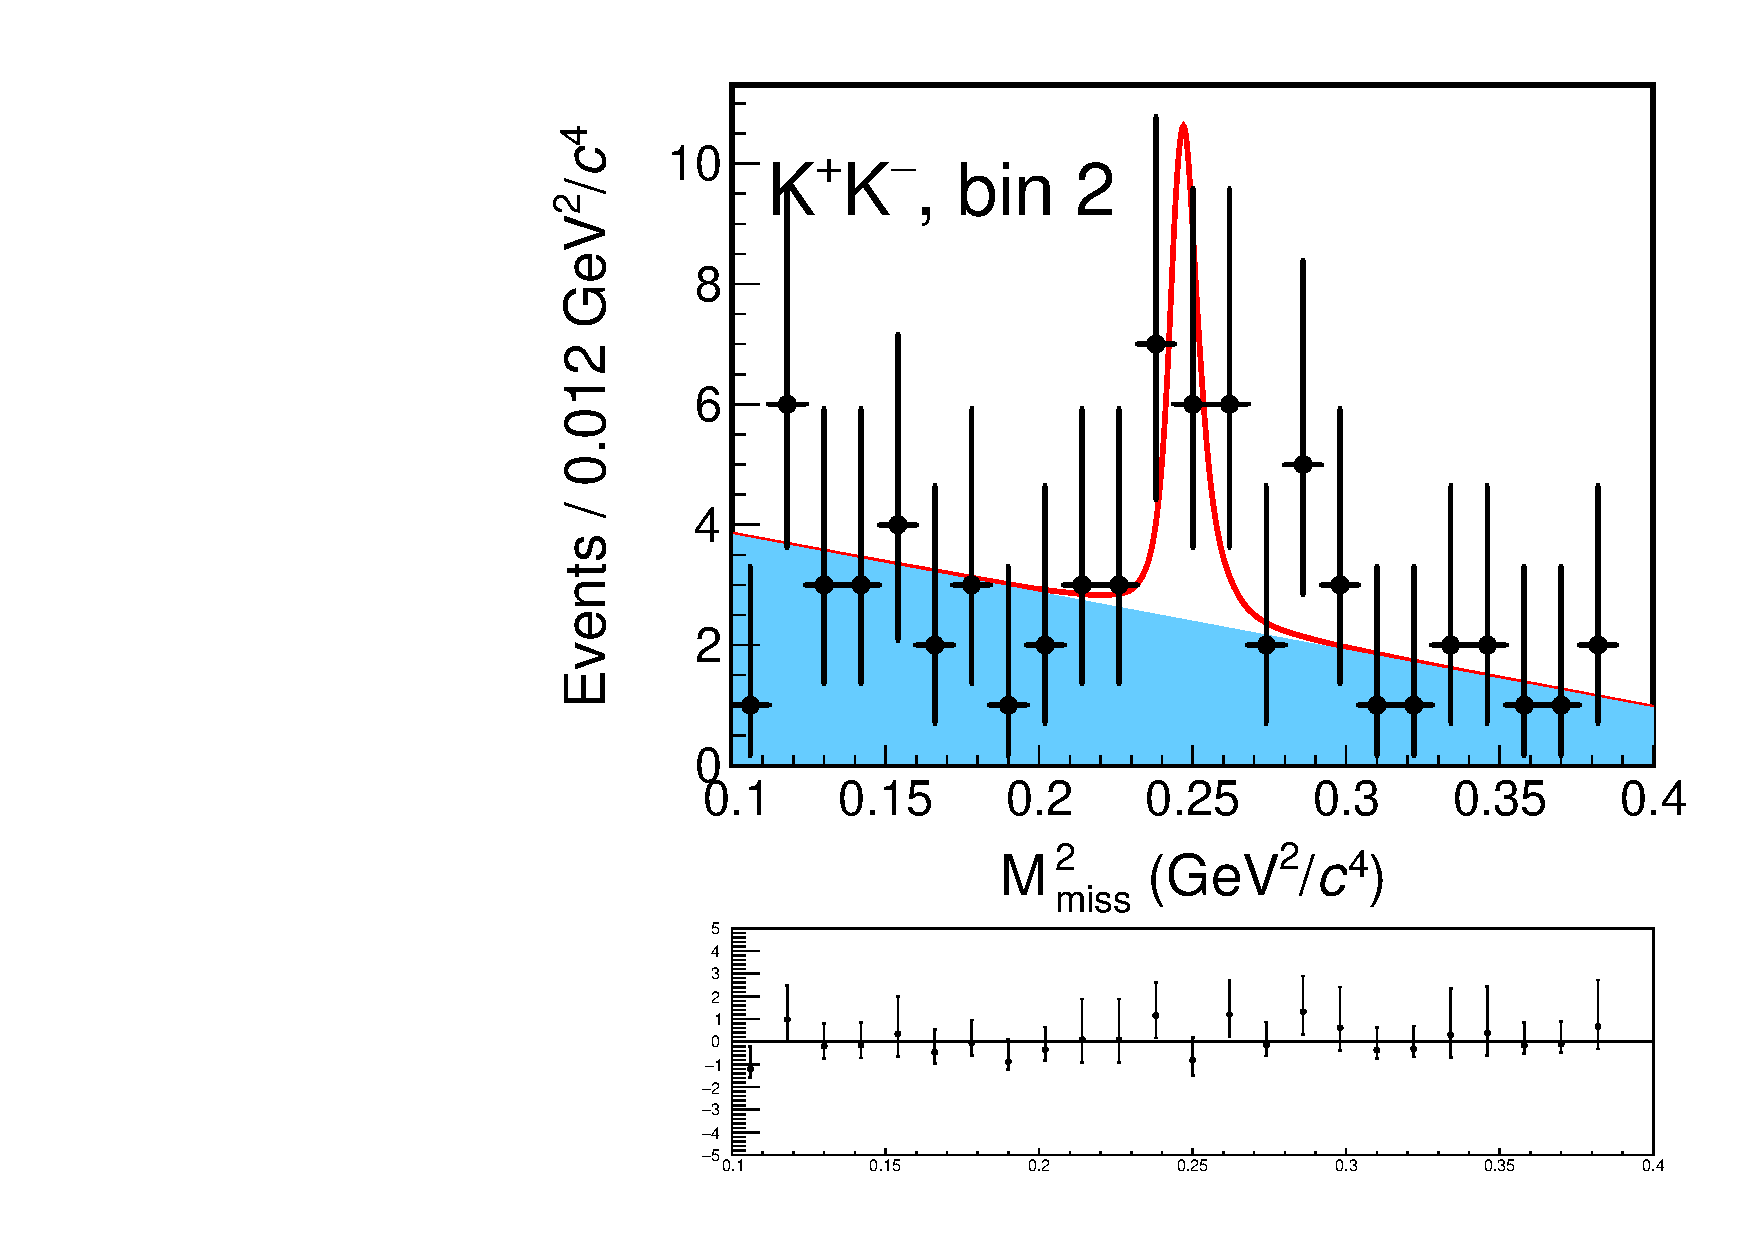
\includegraphics[width = 1.0\textwidth,trim={0 5cm 0 0},clip=true]{Plots/DoubleTagYield_DoubleTag_CP_KKpipi_vs_KKPartReco_SignalBin2.pdf}
      \caption{Bin 2, $N^{\rm DT} = 10.1^{+5.1}_{-4.2}$}
    \end{subfigure}
    \caption{Double tag fit of partially reconstructed $KK\pi\pi$ vs $KK$}
  \end{figure}
\end{frame}

\begin{frame}{Double tag yields of partially reconstructed events}
  \begin{center}
    Finally, I can run the fit and the yields were found to be similar to the fully reconstructed samples
  \end{center}
  \begin{figure}
    \centering
    \begin{subfigure}{0.4\textwidth}
      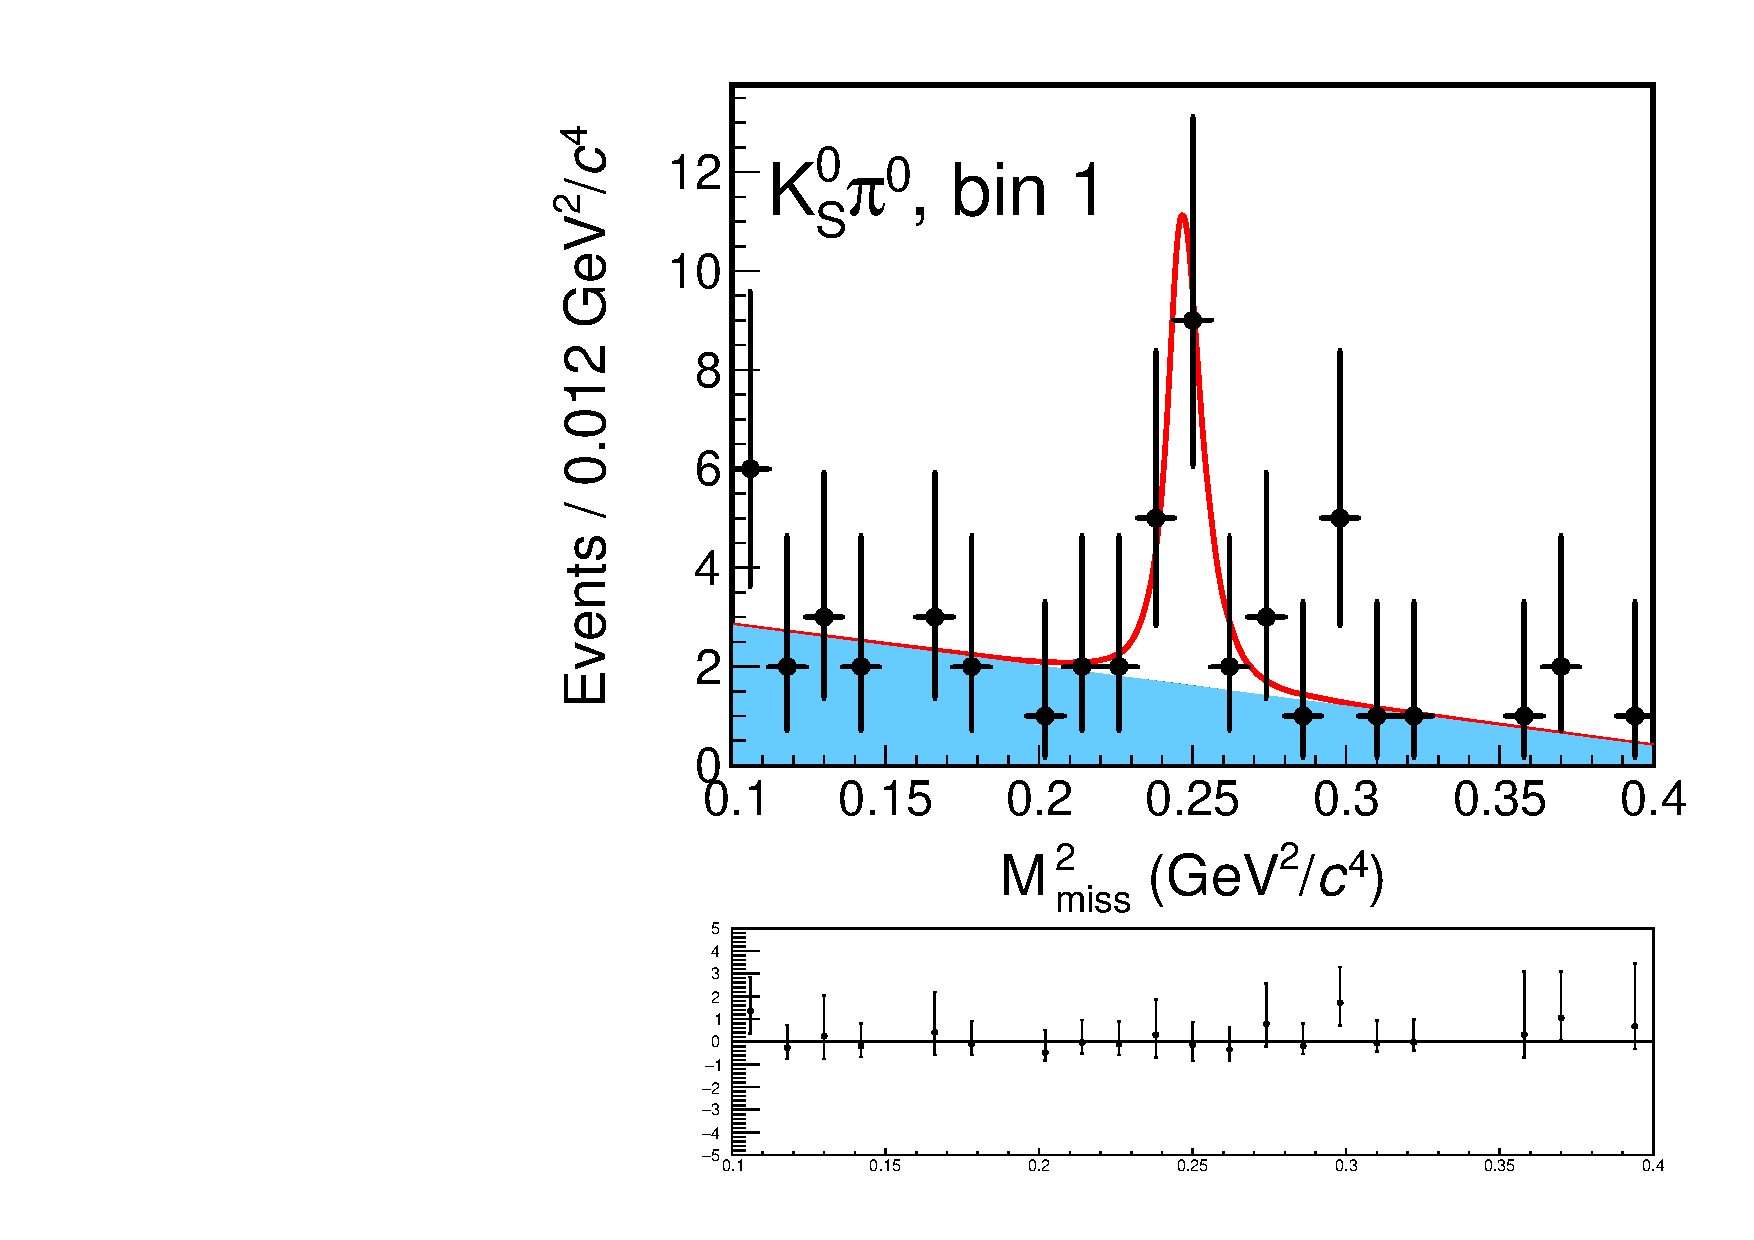
\includegraphics[width = 1.0\textwidth,trim={0 5cm 0 0},clip=true]{Plots/DoubleTagYield_DoubleTag_CP_KKpipi_vs_KSpi0PartReco_SignalBin1.pdf}
      \caption{Bin 1, $N^{\rm DT} = 13.8^{+5.0}_{-4.2}$}
    \end{subfigure}%
    \begin{subfigure}{0.4\textwidth}
      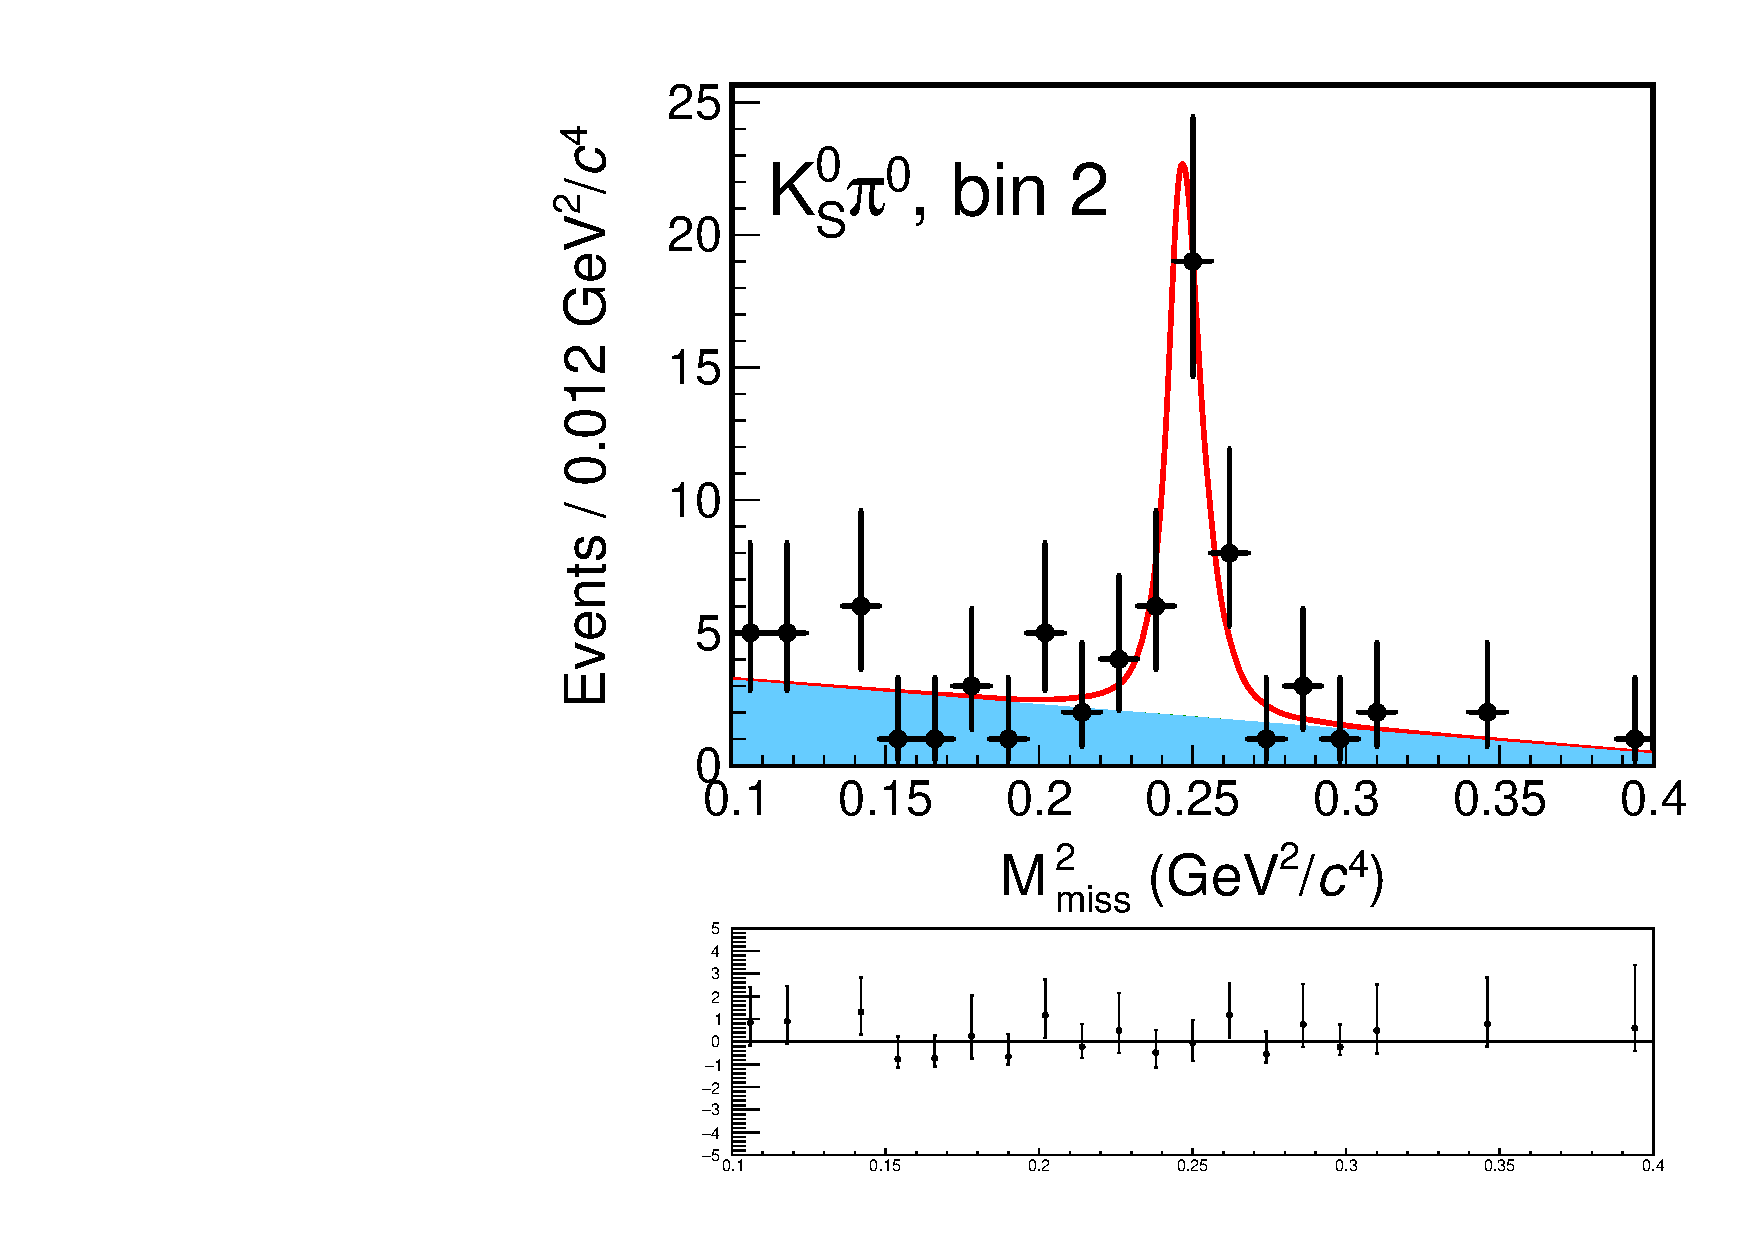
\includegraphics[width = 1.0\textwidth,trim={0 5cm 0 0},clip=true]{Plots/DoubleTagYield_DoubleTag_CP_KKpipi_vs_KSpi0PartReco_SignalBin2.pdf}
      \caption{Bin 2, $N^{\rm DT} = 30.2^{+6.9}_{-6.2}$}
    \end{subfigure}
    \caption{Double tag fit of partially reconstructed $KK\pi\pi$ vs $K_S\pi^0$}
  \end{figure}
\end{frame}

\begin{frame}{Double tag yields of partially reconstructed events}
  \begin{center}
    Partially reconstructed $KK\pi\pi$ vs $\pi\pi\pi^0$ mode not understood yet...\\
    Probably background from light hadrons, such as $e^+e^-\to K_1\bar{K^*}\rho\to KK\pi\pi\pi\pi\pi^0$
  \end{center}
  \begin{figure}
    \centering
    \begin{subfigure}{0.4\textwidth}
      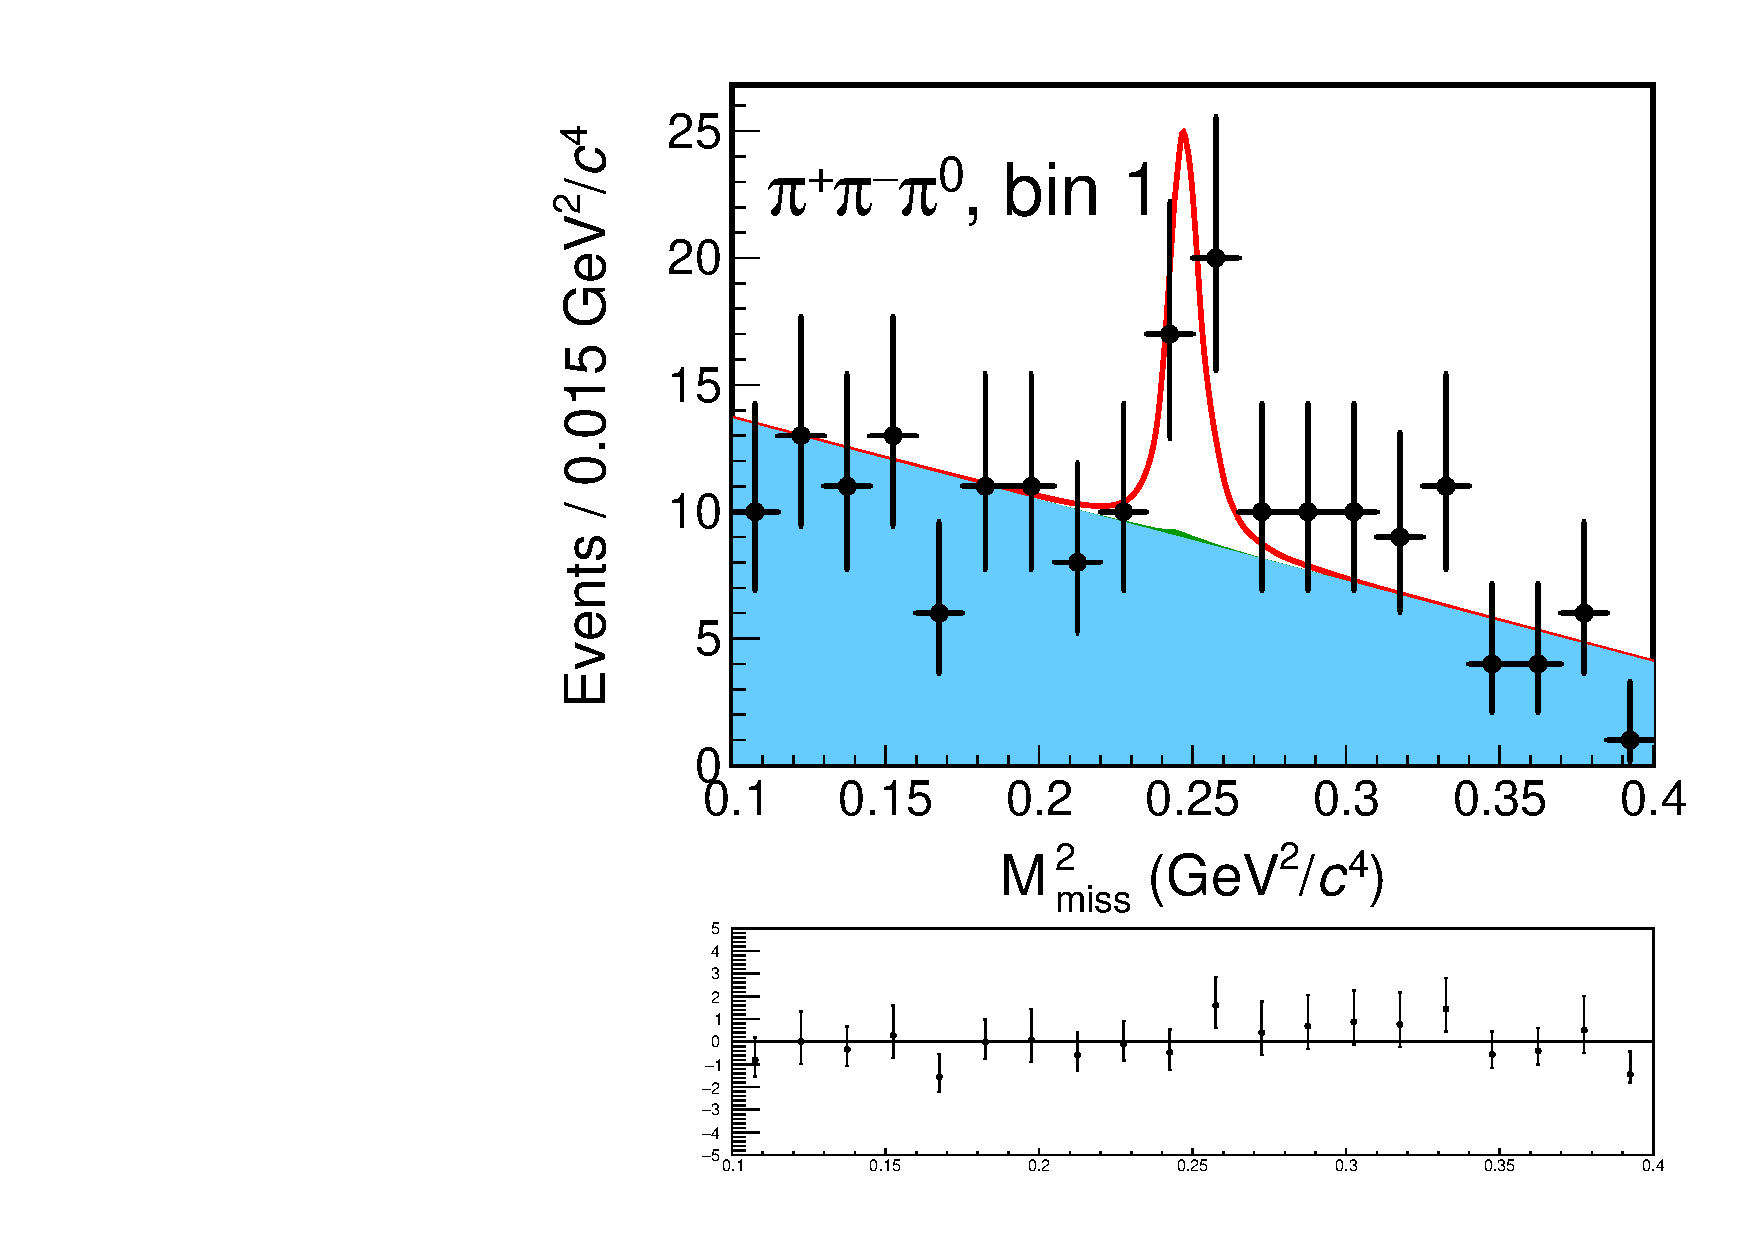
\includegraphics[width = 1.0\textwidth,trim={0 5cm 0 0},clip=true]{Plots/DoubleTagYield_DoubleTag_CP_KKpipi_vs_pipipi0PartReco_SignalBin1.pdf}
      \caption{Bin 1}
    \end{subfigure}%
    \begin{subfigure}{0.4\textwidth}
      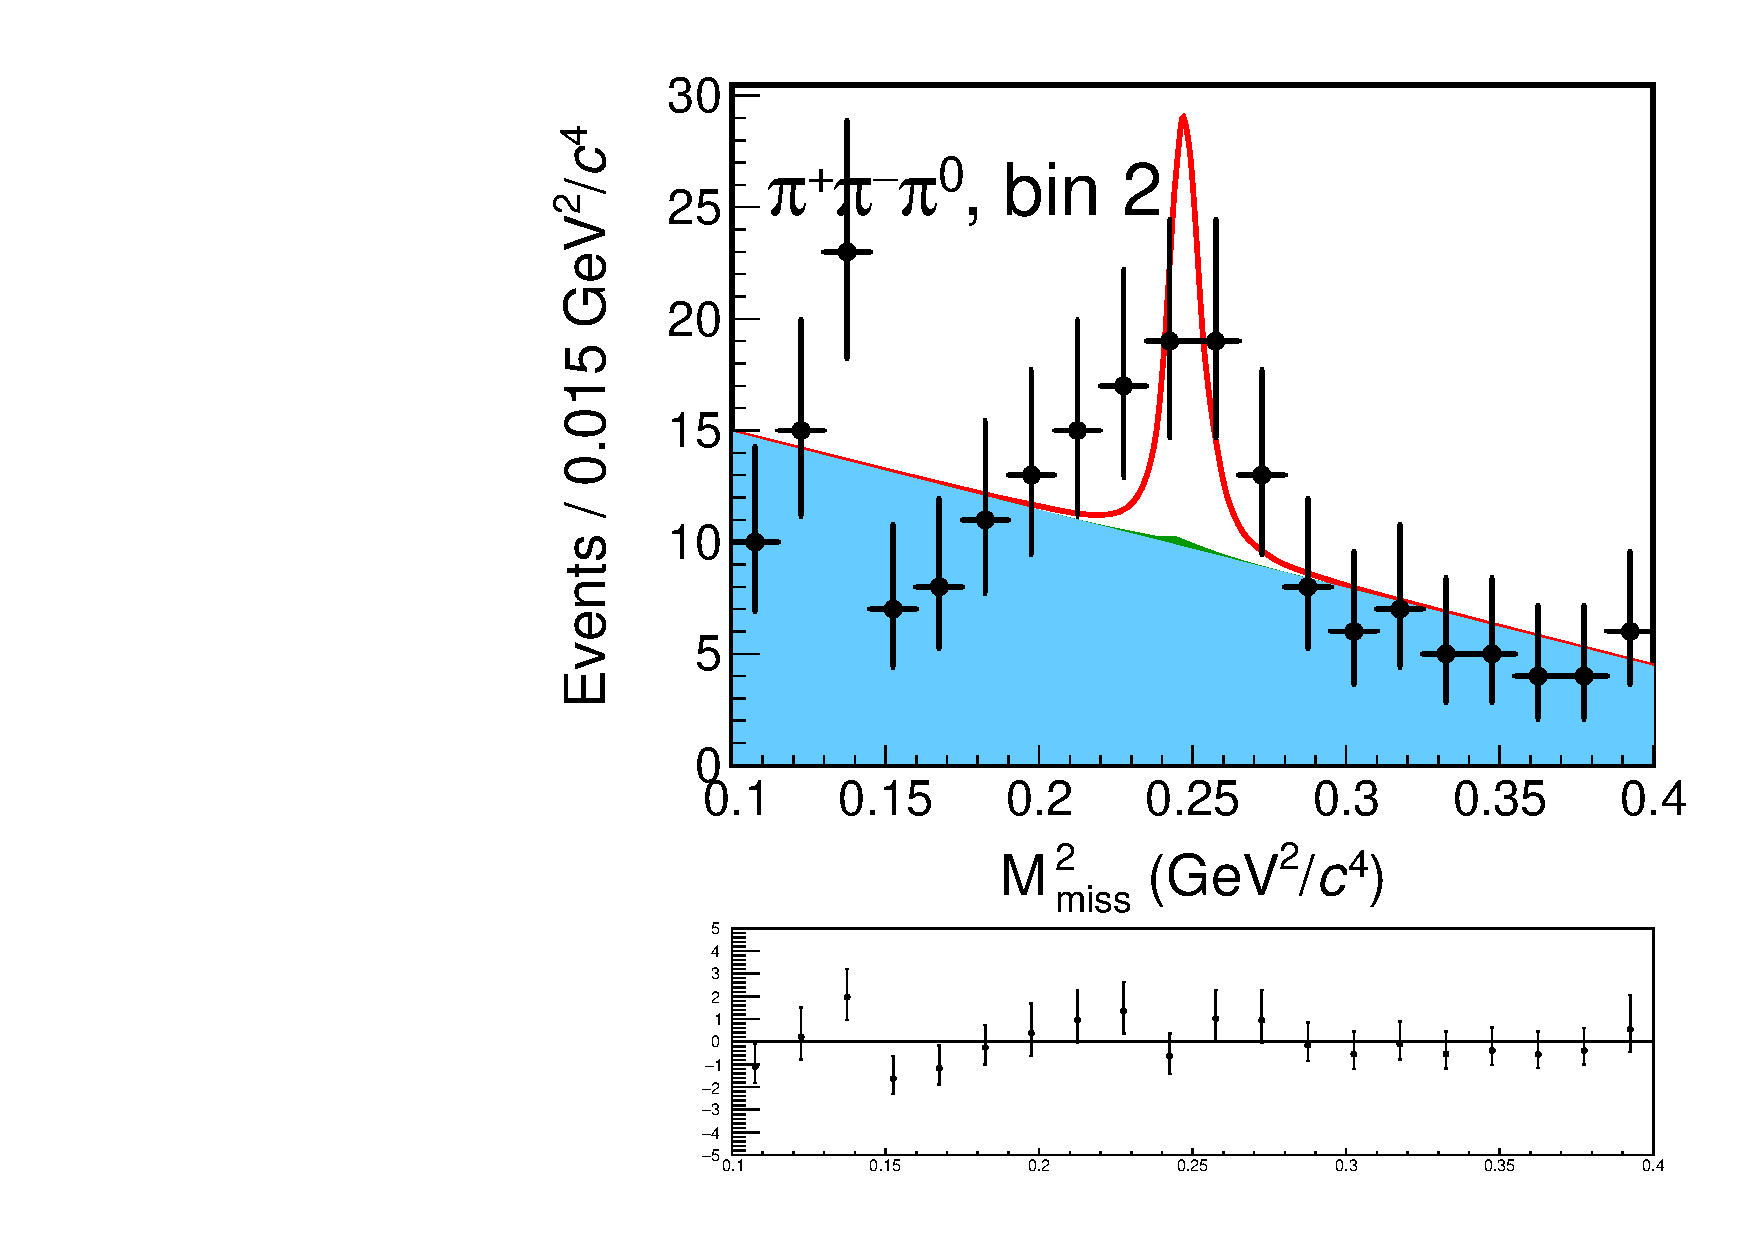
\includegraphics[width = 1.0\textwidth,trim={0 5cm 0 0},clip=true]{Plots/DoubleTagYield_DoubleTag_CP_KKpipi_vs_pipipi0PartReco_SignalBin2.pdf}
      \caption{Bin 2}
    \end{subfigure}
    \caption{Double tag fit of partially reconstructed $KK\pi\pi$ vs $\pi\pi\pi^0$}
  \end{figure}
\end{frame}

\section{\texorpdfstring{$c_i$ and $s_i$}{ci and si} fit}
\begin{frame}{$c_i$ and $s_i$ fit}
  \begin{center}
    {\huge $c_i$ and $s_i$ fit}
  \end{center}
\end{frame}

\begin{frame}{$c_i$ and $s_i$ fit}
  \begin{block}{\centering Equations for $c_i$ and $s_i$}
    \begin{center}
      $\frac{N^{\rm DT}_i}{N^{\rm ST}} = \mathcal{B}(KK\pi\pi)\times(K_i + \bar{K_i} \pm 2\sqrt{K_i\bar{K_i}}c_i)$ \\
      $\frac{N^{\rm DT}_{ij}}{N^{\rm ST}} = \mathcal{B}(KK\pi\pi)\times\big(K_i\bar{K_j'} + \bar{K_i}K_j' - 2\sqrt{K_i\bar{K_i}K_j'\bar{K_j'}}(c_ic_j' + s_is_j')\big)$
    \end{center}
  \end{block}
  \begin{center}
    Fit setup:
  \end{center}
  \begin{enumerate}
    \setlength\itemsep{1.0em}
    \item{$K_i$ and $N^{\rm ST}$ are fixed, apply systematic or Gaussian constrain}
    \item{$\mathcal{B}(KK\pi\pi)$, $c_i$ and $s_i$ are floating}
    \item{Construct likelihood from DT yields and their (asymmetric) uncertainties, using the equations above}
    \item{Correct $K_i$ for DCS decays \underline{directly in the fit}}
  \end{enumerate}
\end{frame}

\begin{frame}{$c_i$ and $s_i$ fit}
  \begin{itemize}
    \item{What are DCS corrections?}
    \begin{itemize}
      \item{Naively, we expect a $K^-\pi^+$ to originate from $D^0$ (CF mode)}
      \item{Therefore the other decay must be $\bar{D^0}\to KK\pi\pi$}
    \end{itemize}
  \end{itemize}
  \begin{figure}[H]
    \centering
    \vspace{0.3cm}
    \begin{fmffile}{fgraph/fgraph_flavour_tag_DCS1}
      \setlength{\unitlength}{1cm}
      \begin{fmfgraph*}(8,4)
        \fmfstraight
        \fmfleft{i4,i3,i2,i1}
        \fmfright{g1,o1,o2,g2}
        \fmflabel{$\pi^+$}{o1}
        \fmflabel{$K^-$}{o2}
        \fmflabel{$K^+$}{i1}
        \fmflabel{$K^-$}{i2}
        \fmflabel{$\pi^+$}{i3}
        \fmflabel{$\pi^-$}{i4}
        \fmf{fermion}{w1,i1}
        \fmf{fermion}{w1,i2}
        \fmf{fermion}{w1,i3}
        \fmf{fermion}{w1,i4}
        \fmf{phantom,tension=5}{w1,w2}
        \fmf{fermion}{w2,o1}
        \fmf{fermion}{w2,o2}
        \fmf{phantom}{w2,g1}
        \fmf{phantom}{w2,g2}
        \fmfblob{0.5cm}{w1}
        \fmfv{label=$\bar{D^0}$,right,label.dist=0.5cm,label.angle=90.0}{w1}
        \fmfblob{0.5cm}{w2}
        \fmfv{label=$D^0$,label.dist=0.5cm,label.angle=90.0}{w2}
      \end{fmfgraph*}
    \end{fmffile}
    \vspace{0.3cm}
  \end{figure}
\end{frame}

\begin{frame}{$c_i$ and $s_i$ fit}
  \begin{itemize}
    \item{What are DCS corrections?}
    \begin{itemize}
      \item{But what if $D^0\to K^+\pi^-$ (DCS mode)?}
      \item{This leads to a bias in $K_i$ because the flavour of $D\to KK\pi\pi$ is wrong}
    \end{itemize}
  \end{itemize}
  \begin{figure}[H]
    \centering
    \vspace{0.3cm}
    \begin{fmffile}{fgraph/fgraph_flavour_tag_DCS2}
      \setlength{\unitlength}{1cm}
      \begin{fmfgraph*}(8,4)
        \fmfstraight
        \fmfleft{i4,i3,i2,i1}
        \fmfright{g1,o1,o2,g2}
        \fmflabel{$\pi^-$}{o1}
        \fmflabel{$K^+$}{o2}
        \fmflabel{$K^+$}{i1}
        \fmflabel{$K^-$}{i2}
        \fmflabel{$\pi^+$}{i3}
        \fmflabel{$\pi^-$}{i4}
        \fmf{fermion}{w1,i1}
        \fmf{fermion}{w1,i2}
        \fmf{fermion}{w1,i3}
        \fmf{fermion}{w1,i4}
        \fmf{phantom,tension=5}{w1,w2}
        \fmf{fermion}{w2,o1}
        \fmf{fermion}{w2,o2}
        \fmf{phantom}{w2,g1}
        \fmf{phantom}{w2,g2}
        \fmfblob{0.5cm}{w1}
        \fmfv{label=$\bar{D^0}$,right,label.dist=0.5cm,label.angle=90.0}{w1}
        \fmfblob{0.5cm}{w2}
        \fmfv{label=$D^0$,label.dist=0.5cm,label.angle=90.0}{w2}
      \end{fmfgraph*}
    \end{fmffile}
    \vspace{0.3cm}
  \end{figure}
\end{frame}

\begin{frame}{$c_i$ and $s_i$ fit}
  \begin{itemize}
    \setlength\itemsep{1.0em}
    \item{Since $|\mathcal{A}(CF)| = r_D|\mathcal{A}(DCS)|$, where $r_D\approx5\%$, DCS decays are suppressed by $r_D^2=\mathcal{O}(10^{-3})$}
    \item{However, since $D\bar{D}$ are quantum correlated, there is an interference!}
    \item{Interference depends on the CF/DCS ratio $r_D$, coherence factor $R$ and strong phase $\delta_D$}
    \item{It also depends on $c_i$ and $s_i$, which we are trying to determine...}
  \end{itemize}
  \vspace{0.5cm}
  \begin{center}
    {\Large The true $K_i$ has contributions from CF and DCS decays, and their interference:}\\~\\
    $K_i^{\rm true} = K_i^{\rm obs} + r_D^2\bar{K_i}^{\rm obs} - 2r_DR\sqrt{K_i^{\rm obs}\bar{K_i^{\rm obs}}}\big(c_i\cos(\delta_D) - s_i\sin(\delta_D)\big)$
  \end{center}
\end{frame}

\begin{frame}{$c_i$ and $s_i$ fit}
  \begin{center}
    {\Large DCS correction factors:}\\~\\
    $f_i = \frac{1}{1 + r_D^2\frac{\bar{K_i}^{\rm obs}}{K_i^{\rm obs}} - 2r_DR\sqrt{\frac{\bar{K_i^{\rm obs}}}{K_i^{\rm obs}}}\big(c_i\cos(\delta_D) - s_i\sin(\delta_D)\big)}$
  \end{center}
  \begin{itemize}
    \setlength\itemsep{1.0em}
    \item{In previous analyses of $D\to K_S\pi\pi$ and $K_SKK$, $f_i$ were calculated using model predictions of $c_i$ and $s_i$}
    \item{Unfortunately, we don't know if the model prediction of $D\to KK\pi\pi$ strong phases is accurate}
    \item{In the $D\to K_S\pi\pi\pi^0$ analysis, only the $D\to Ke\nu$ flavour tag was used, because no amplitude model exists (yet)}
  \end{itemize}
  \begin{center}
    Solution: Add DCS corrections directly into the fit\\
    Calculate $K_i^{\rm true}$, using 3 iterations, with the fitted $c_i$/$s_i$
  \end{center}
\end{frame}

\begin{frame}{$c_i$ and $s_i$ fit}
  \begin{center}
    With this strategy, the fit will determine the DCS corrections for us\\
    Here, using $D\to K\pi$ as an example:
  \end{center}
  \vspace{0.5cm}
  \centering
  \def\arraystretch{1.2}%
  \begin{tabular}{lcc}
    Bin     & $f_i$  & $f_{-i}$ \\
    \hline
    $1$     & $0.95$ & $0.98$ \\
    $2$     & $0.94$ & $0.97$ \\
    \hline
  \end{tabular}
  \vspace{1.0cm}
  \begin{center}
    Bonus measurement: Instead of using the $K\pi$ tag to measure $K_i$, we can actually float $\delta_D^{K\pi}$ directly in the fit, and hence simultaneously measure the strong phase of the $D\to K\pi$ decay!
  \end{center}
\end{frame}

\begin{frame}{$c_i$ and $s_i$ fit}
  \begin{center}
    Perform fit of $c_i$ and $s_i$, using the fully reconstructed $KK$, $\pi\pi\pi^0$, $K_S\pi^0$ and $K_S\pi\pi$ tags, as well as partially reconstructed $KK\pi\pi$ vs $KK$ and $K_S\pi^0$
  \end{center}
  \vspace{-0.3cm}
  \begin{figure}
    \centering
    \begin{subfigure}{0.4\textwidth}
      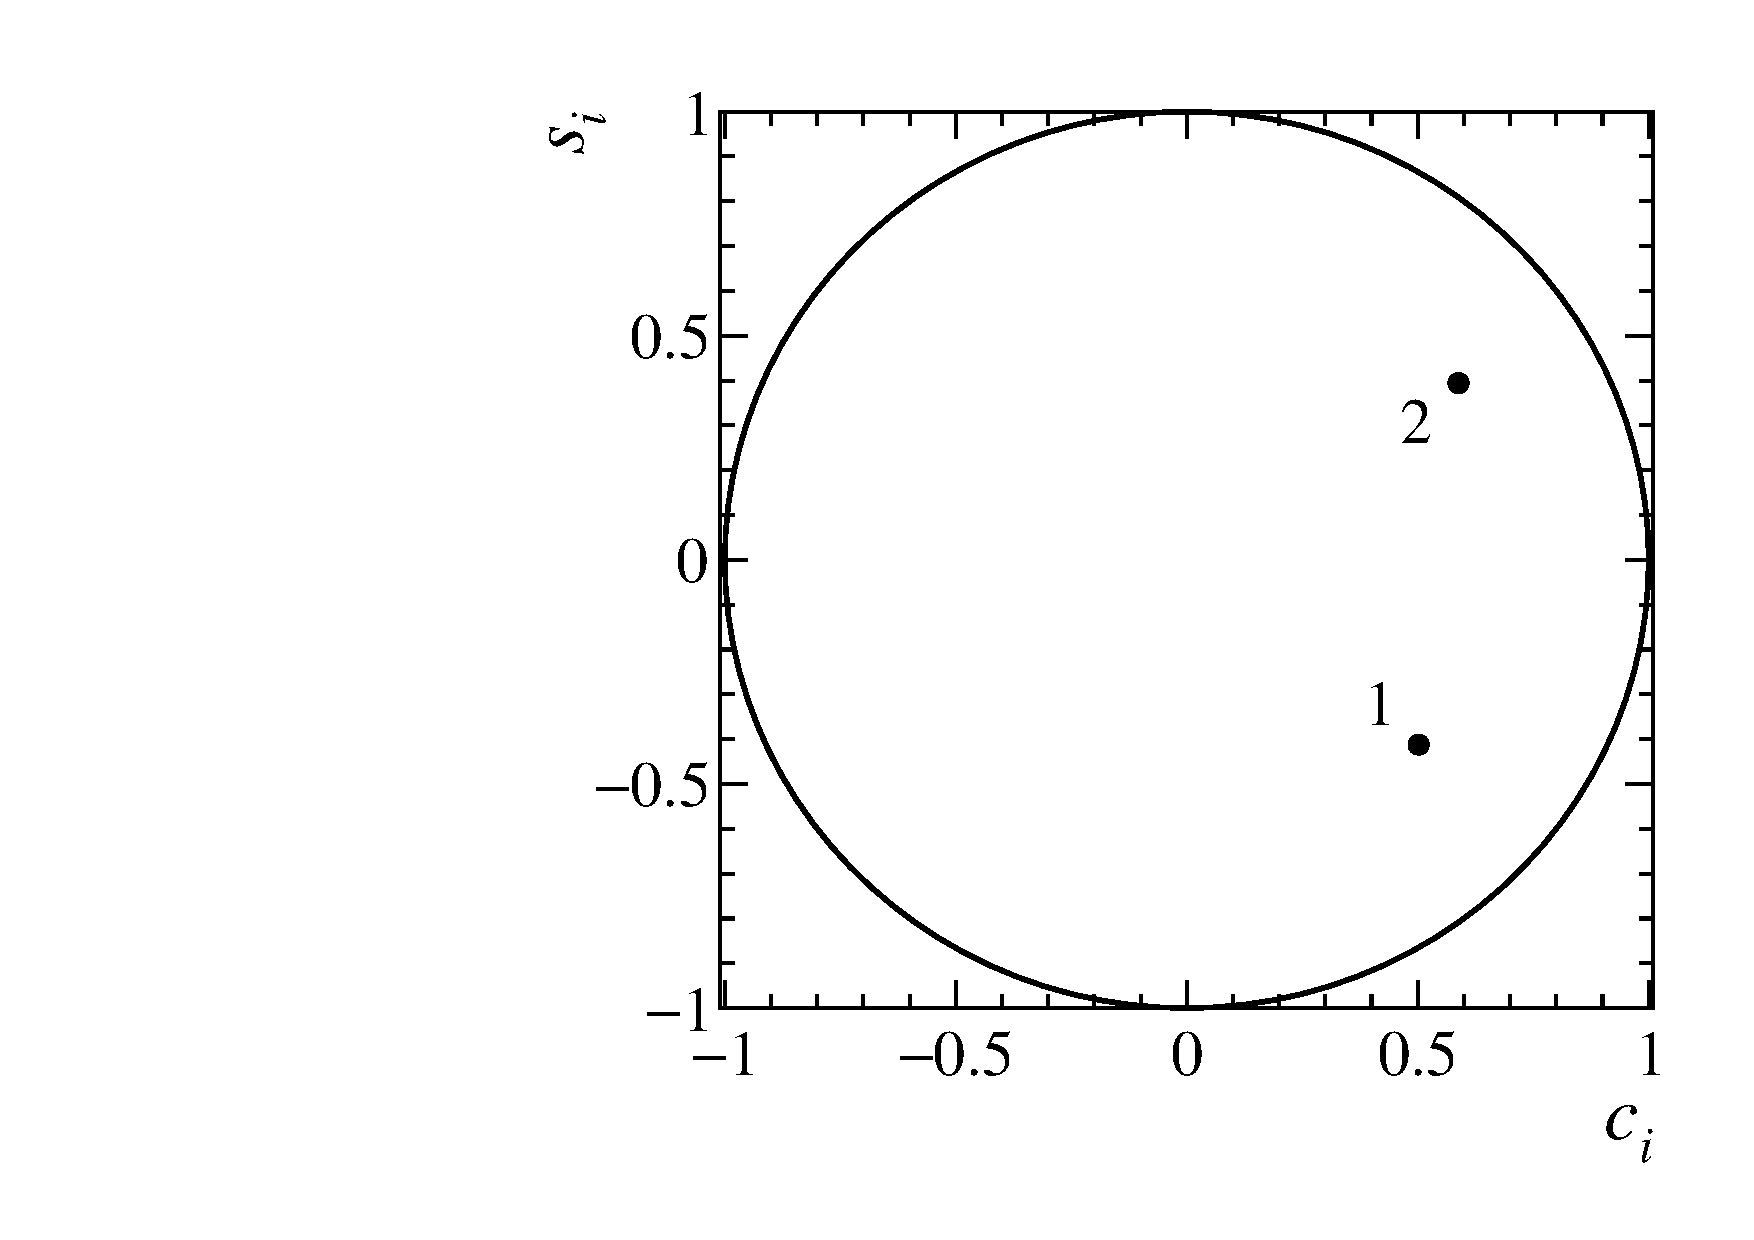
\includegraphics[width = 1.0\textwidth]{Plots/StrongPhaseParametersPlot_cisi_2Bins.pdf}
    \end{subfigure}%
    \begin{subfigure}{0.4\textwidth}
      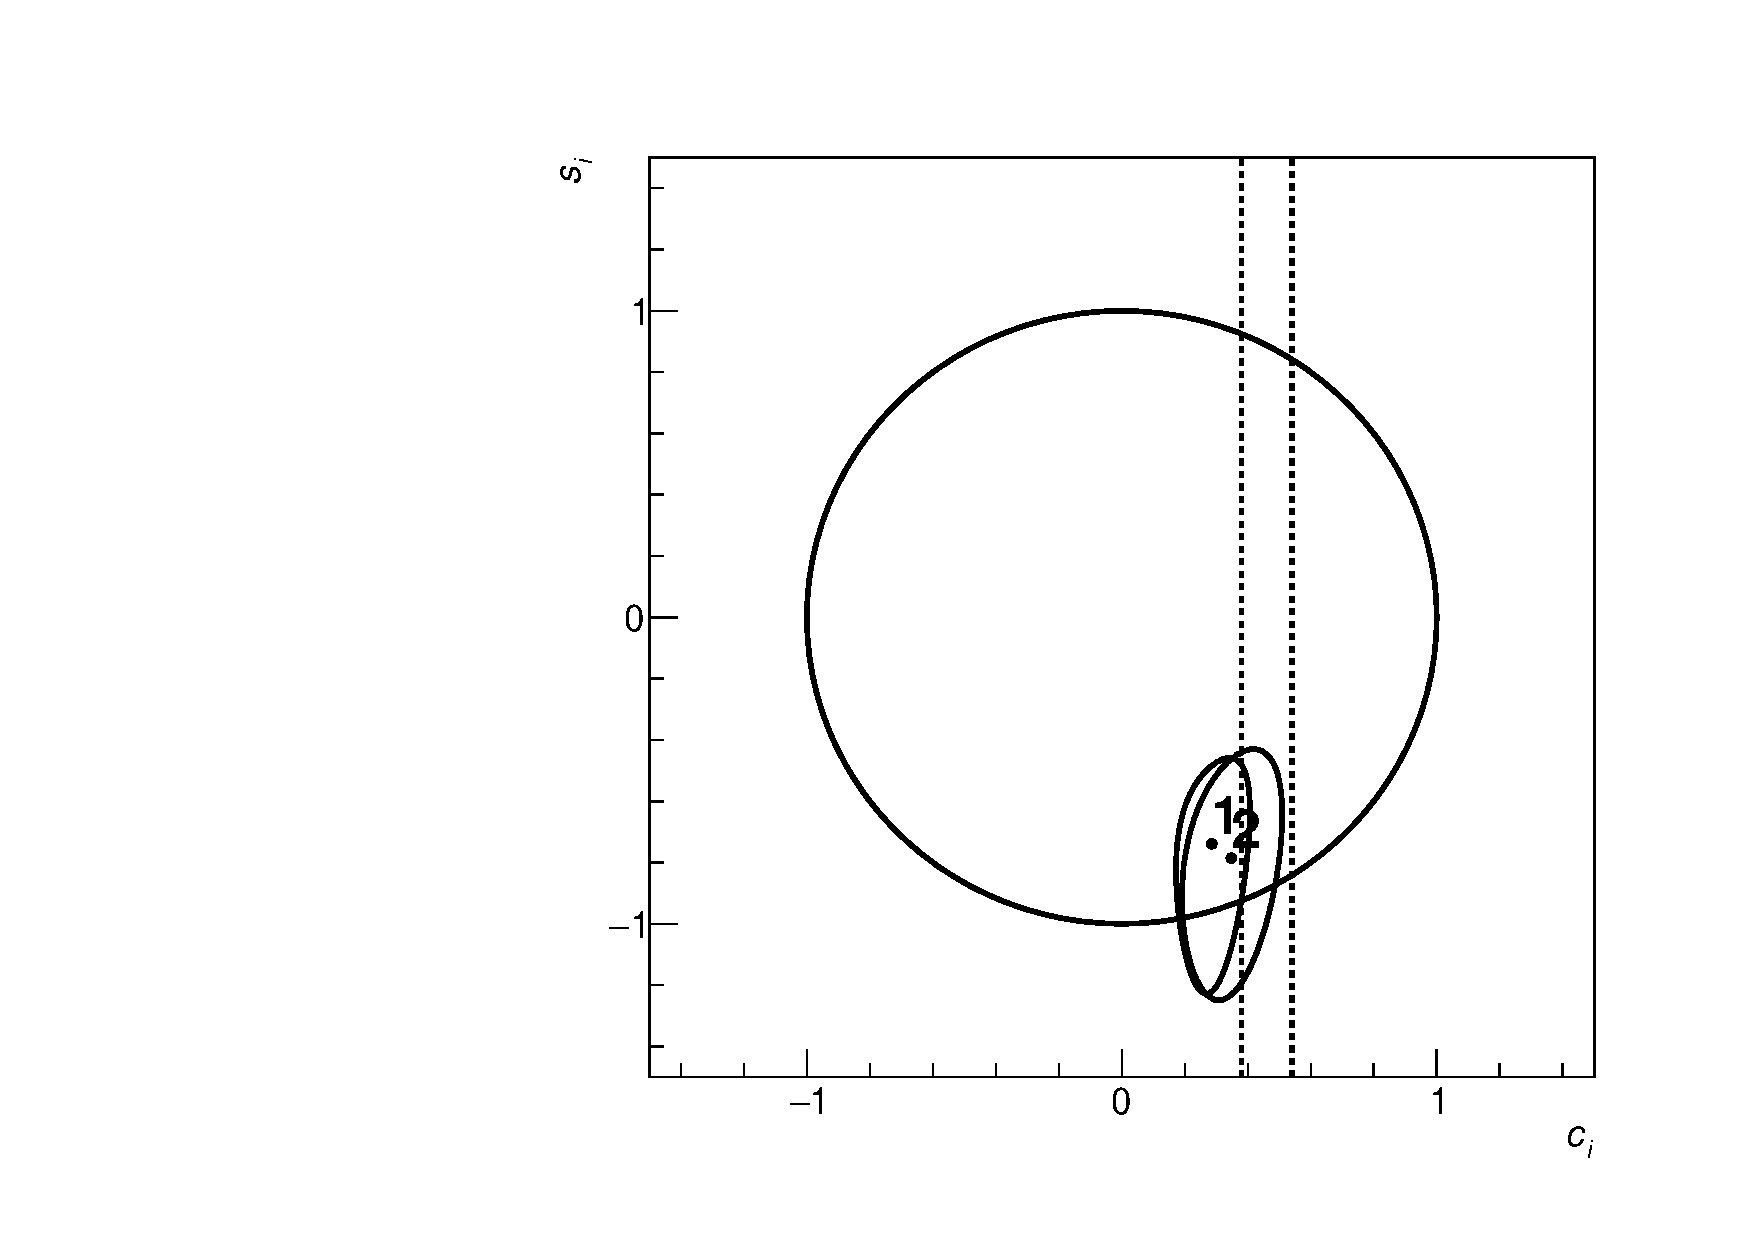
\includegraphics[width = 1.0\textwidth]{Plots/Contours_cisi.pdf}
      \vspace{0.07cm}
    \end{subfigure}
    \vspace{-0.5cm}
    \caption{Comparison of fitted values of $c_i$ and $s_i$ (left), and the model predictions (right)}
  \end{figure}
  \vspace{-0.4cm}
  \begin{center}
    $c_i$ agrees well with $F_+$ measurement (as it should), but $s_i$ clearly shows a tension with the model!
  \end{center}
\end{frame}

\begin{frame}{Summary and next steps}
  \begin{itemize}
    \setlength\itemsep{0.8em}
    \item{BESIII measurement of $c_i$ and $s_i$ is progressing well}
    \item{A partially reconstructed $D\to KK\pi\pi$ method has been tested, but there were some challenges with large $D\to K\pi\pi\pi\pi^0$ backgrounds}
    \item{The preliminary fit of $c_i$ and $s_i$ shows promising results}
    \begin{itemize}
      \item{A method for direct DCS decay corrections is working well}
      \item{Results of $c_i$ agree with the $F_+$ measurement}
      \item{$s_i$ shows tensions with the LHCb model}
    \end{itemize}
    \item{Next steps:}
    \begin{enumerate}
      \item{Finish calculation of peaking backgrounds in each bin}
      \item{Reprocess all data and generate new MC once new data is available}
      \item{Add the rest of the tags}
      \item{Charm WG review}
    \end{enumerate}
  \end{itemize}
  \begin{center}
    \huge Thank you for listening!
  \end{center}
\end{frame}

\section{Backup: Double tag yields of fully reconstructed events}
\begin{frame}{Backup: Double tag yields of fully reconstructed events}
  \begin{center}
    {\huge Backup: Double tag yields of fully reconstructed events}
  \end{center}
\end{frame}

\begin{frame}{Backup: Double tag yields of fully reconstructed events}
  \begin{center}
    Strategy for measuring DT yields of fully reconstructed events:
  \end{center}
  \begin{itemize}
    \setlength\itemsep{0.5em}
    \item{Fit the beam constrained mass $M_{\rm BC} = \sqrt{E_{\rm beam}^2 - \sum_i|\vec{p}_i|^2}$}
    \item{Signal shape: MC-derived shape, convolved with Gaussian}
    \item{Flat background: Argus function}
    \item{Peaking background: Fixed from MC}
  \end{itemize}
  \begin{figure}
    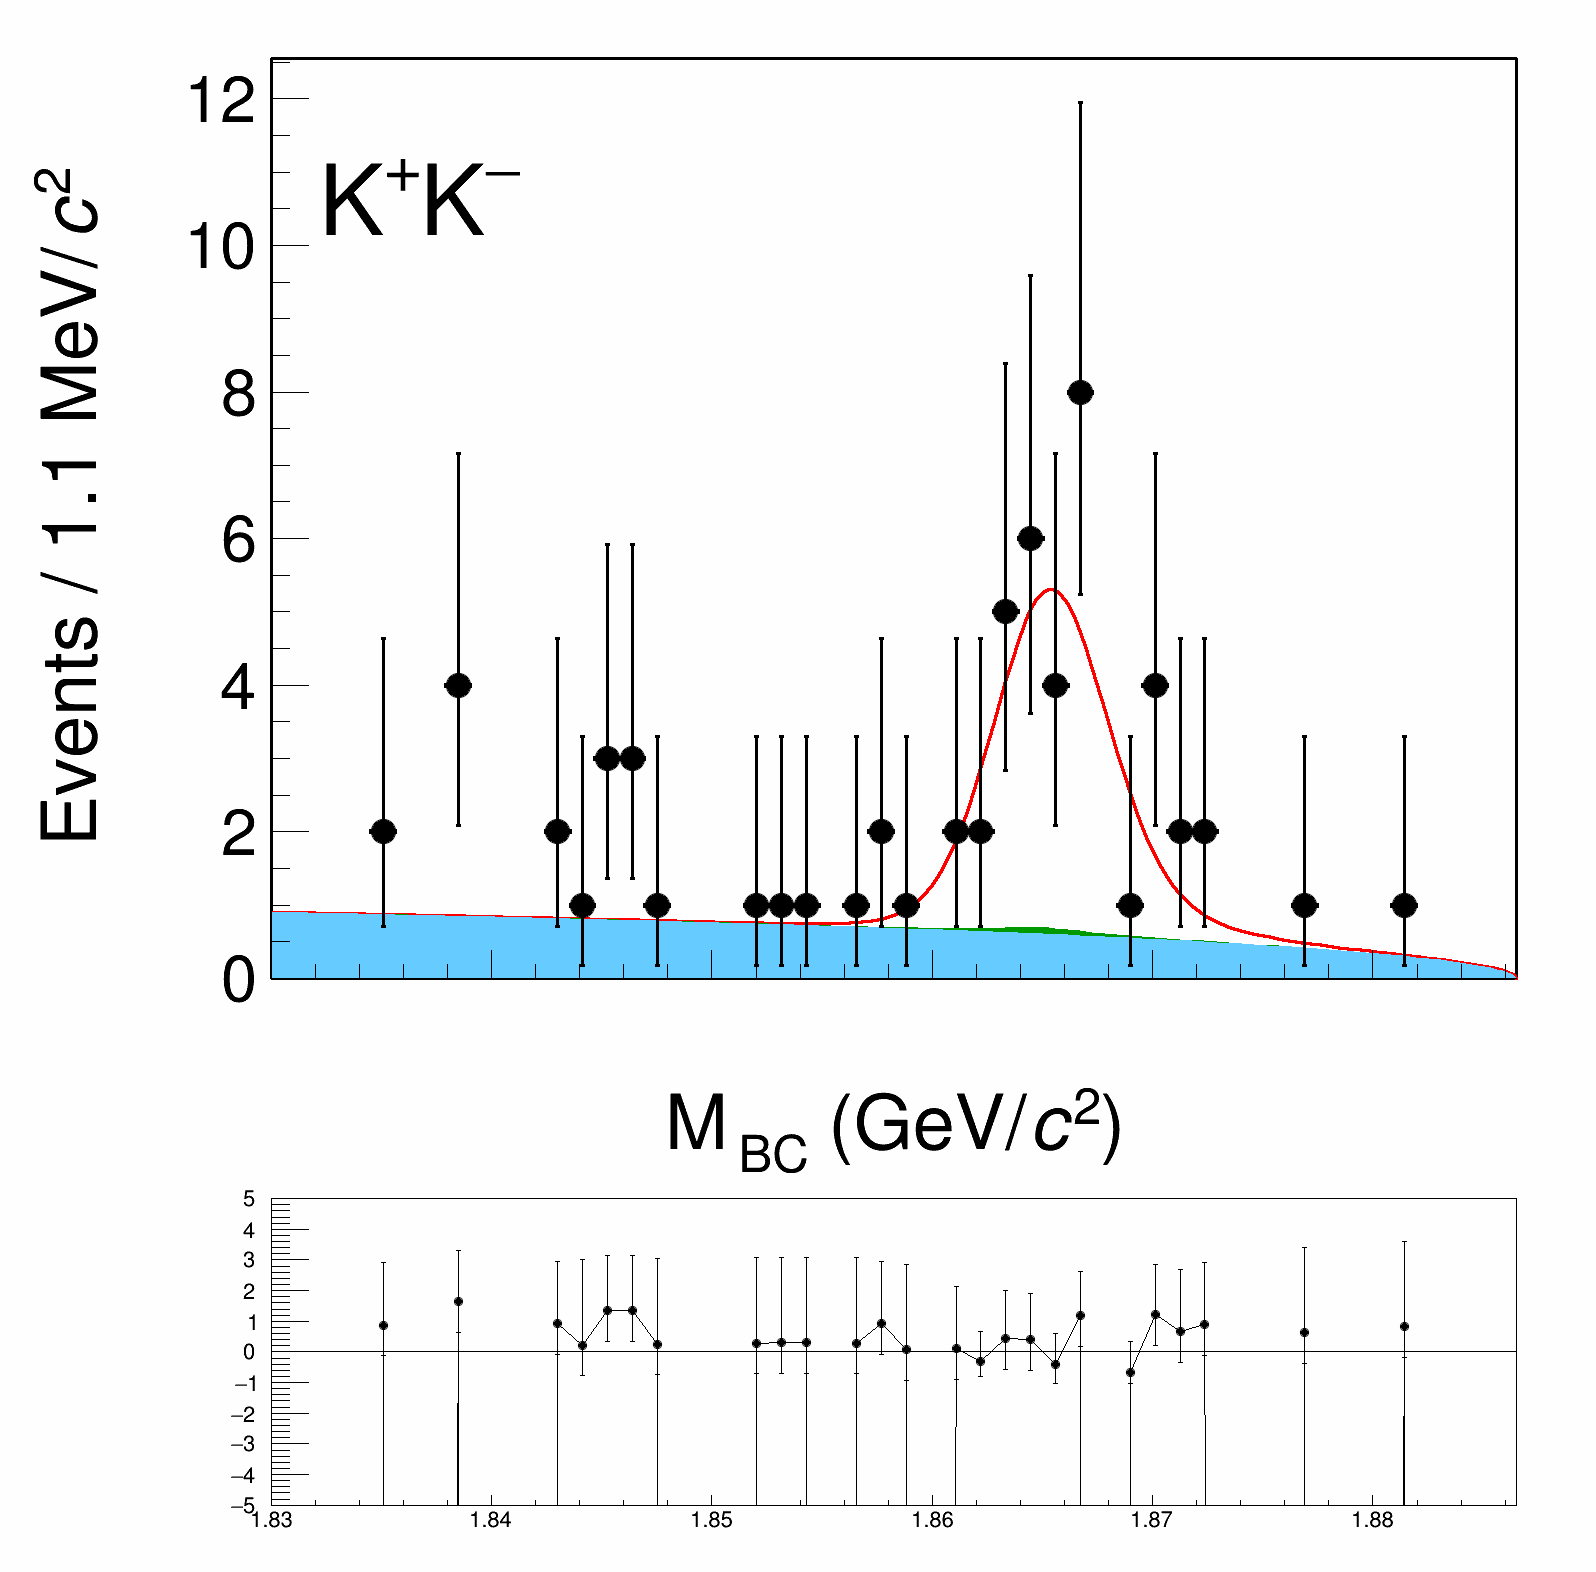
\includegraphics[width = 0.4\textwidth,trim={0 14cm 0 0},clip=true]{Plots/DoubleTagYield_DoubleTag_CP_KKpipi_vs_KK_SignalBin0.png}
    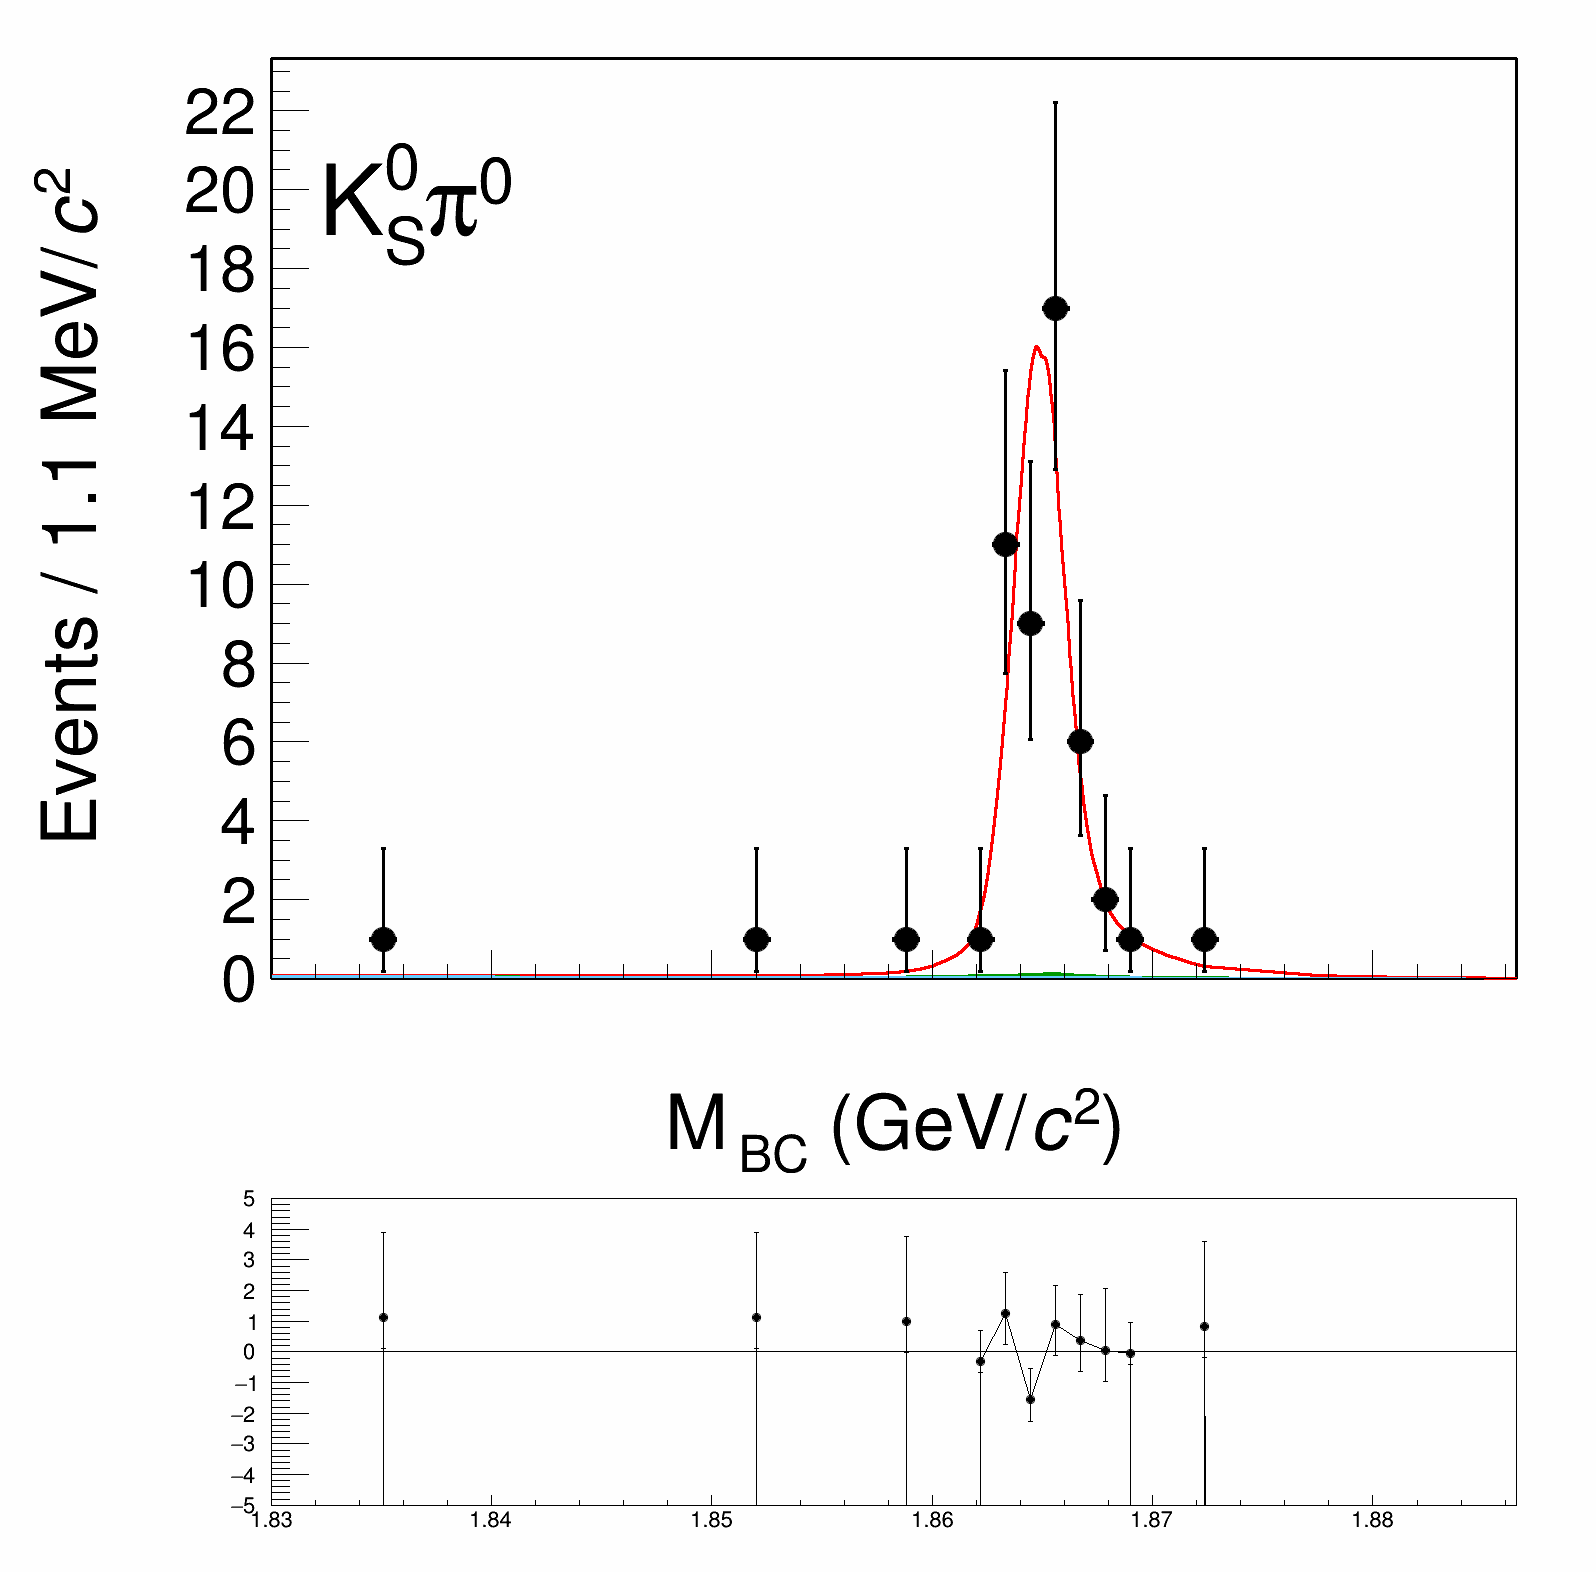
\includegraphics[width = 0.4\textwidth,trim={0 14cm 0 0},clip=true]{Plots/DoubleTagYield_DoubleTag_CP_KKpipi_vs_KSpi0_SignalBin0.png}
  \end{figure}
\end{frame}
    
\begin{frame}{Backup: Double tag yields of fully reconstructed events}
  \begin{center}
    Problem: Fully pionic tag modes have very large backgrounds!
  \end{center}
  \begin{figure}
    \centering
    \begin{subfigure}{0.4\textwidth}
      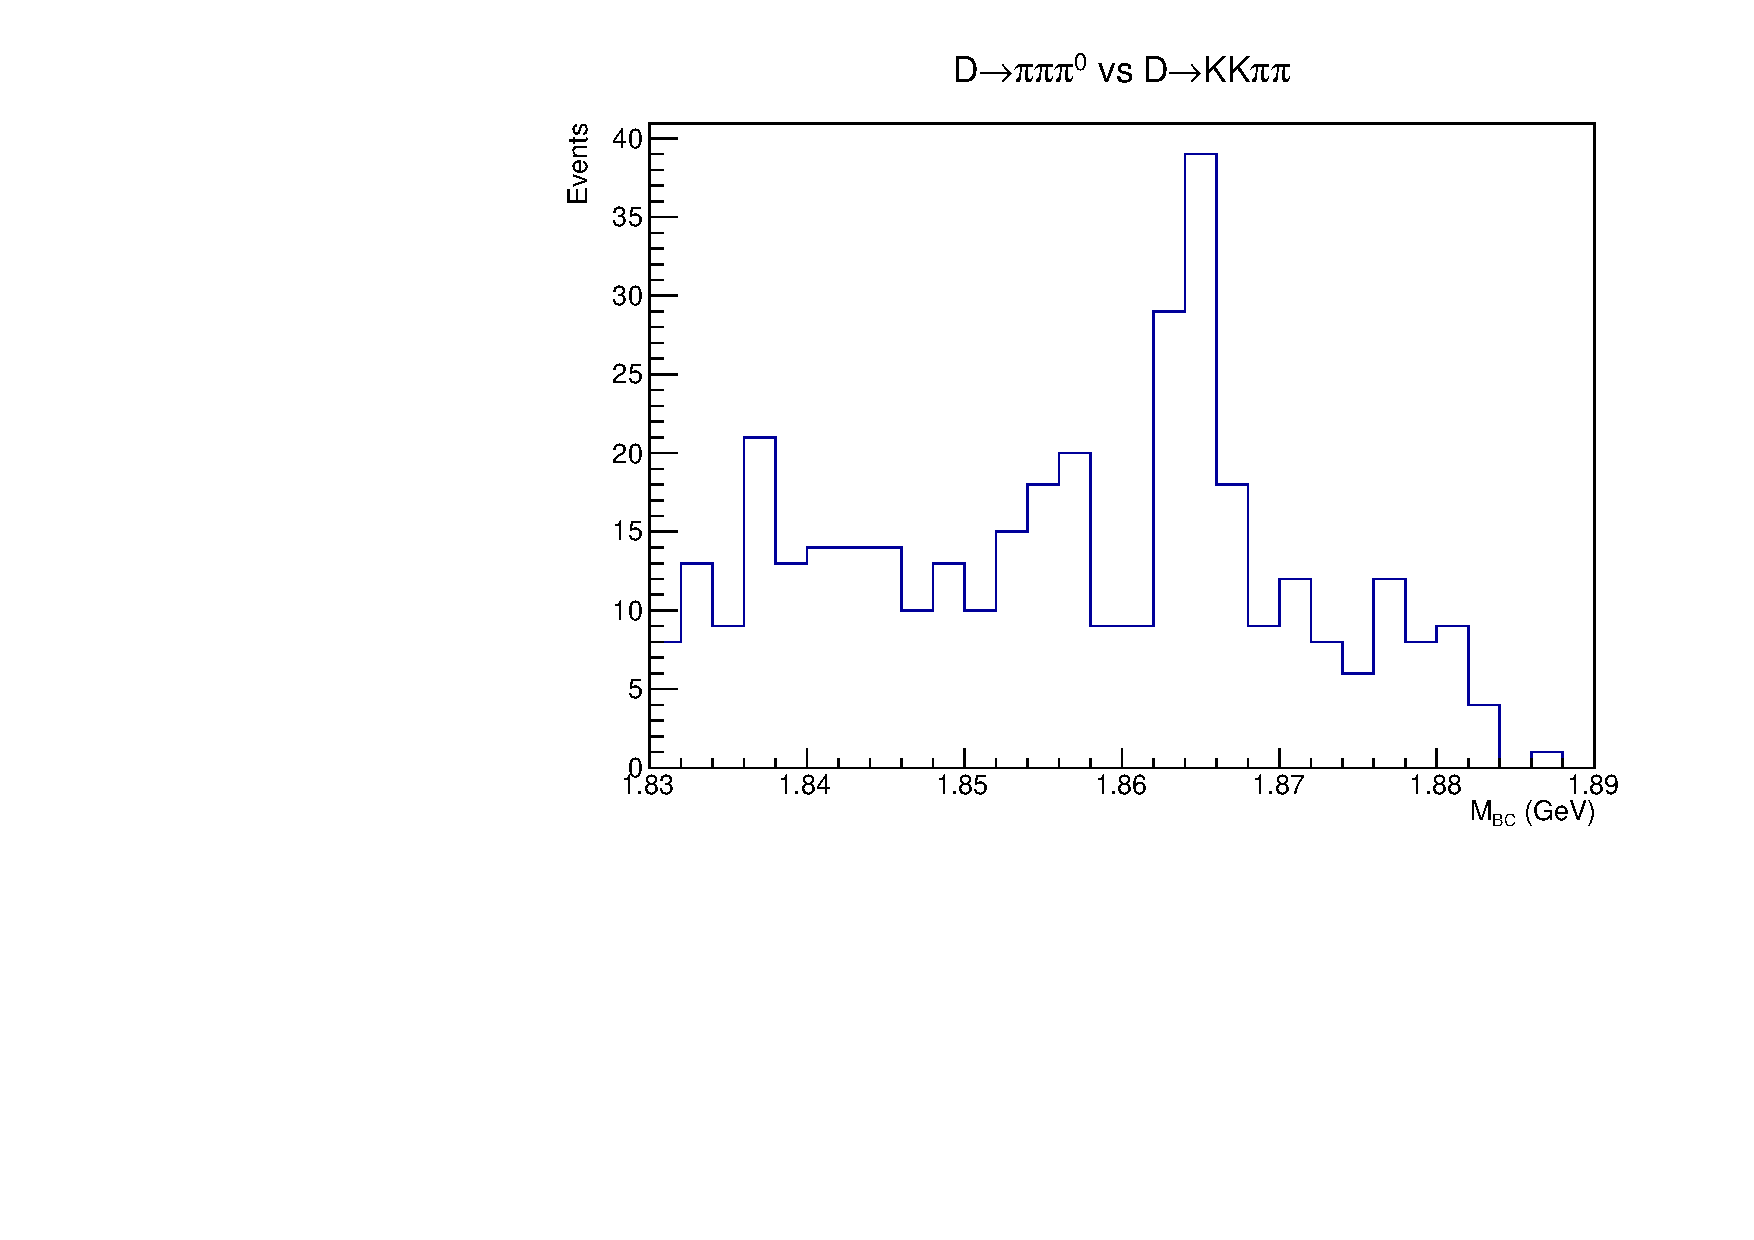
\includegraphics[width = 1.0\textwidth]{Plots/pipipi0_MBC.pdf}
      \caption{$D\to\pi\pi\pi^0$ tag}
    \end{subfigure}%
    \begin{subfigure}{0.4\textwidth}
      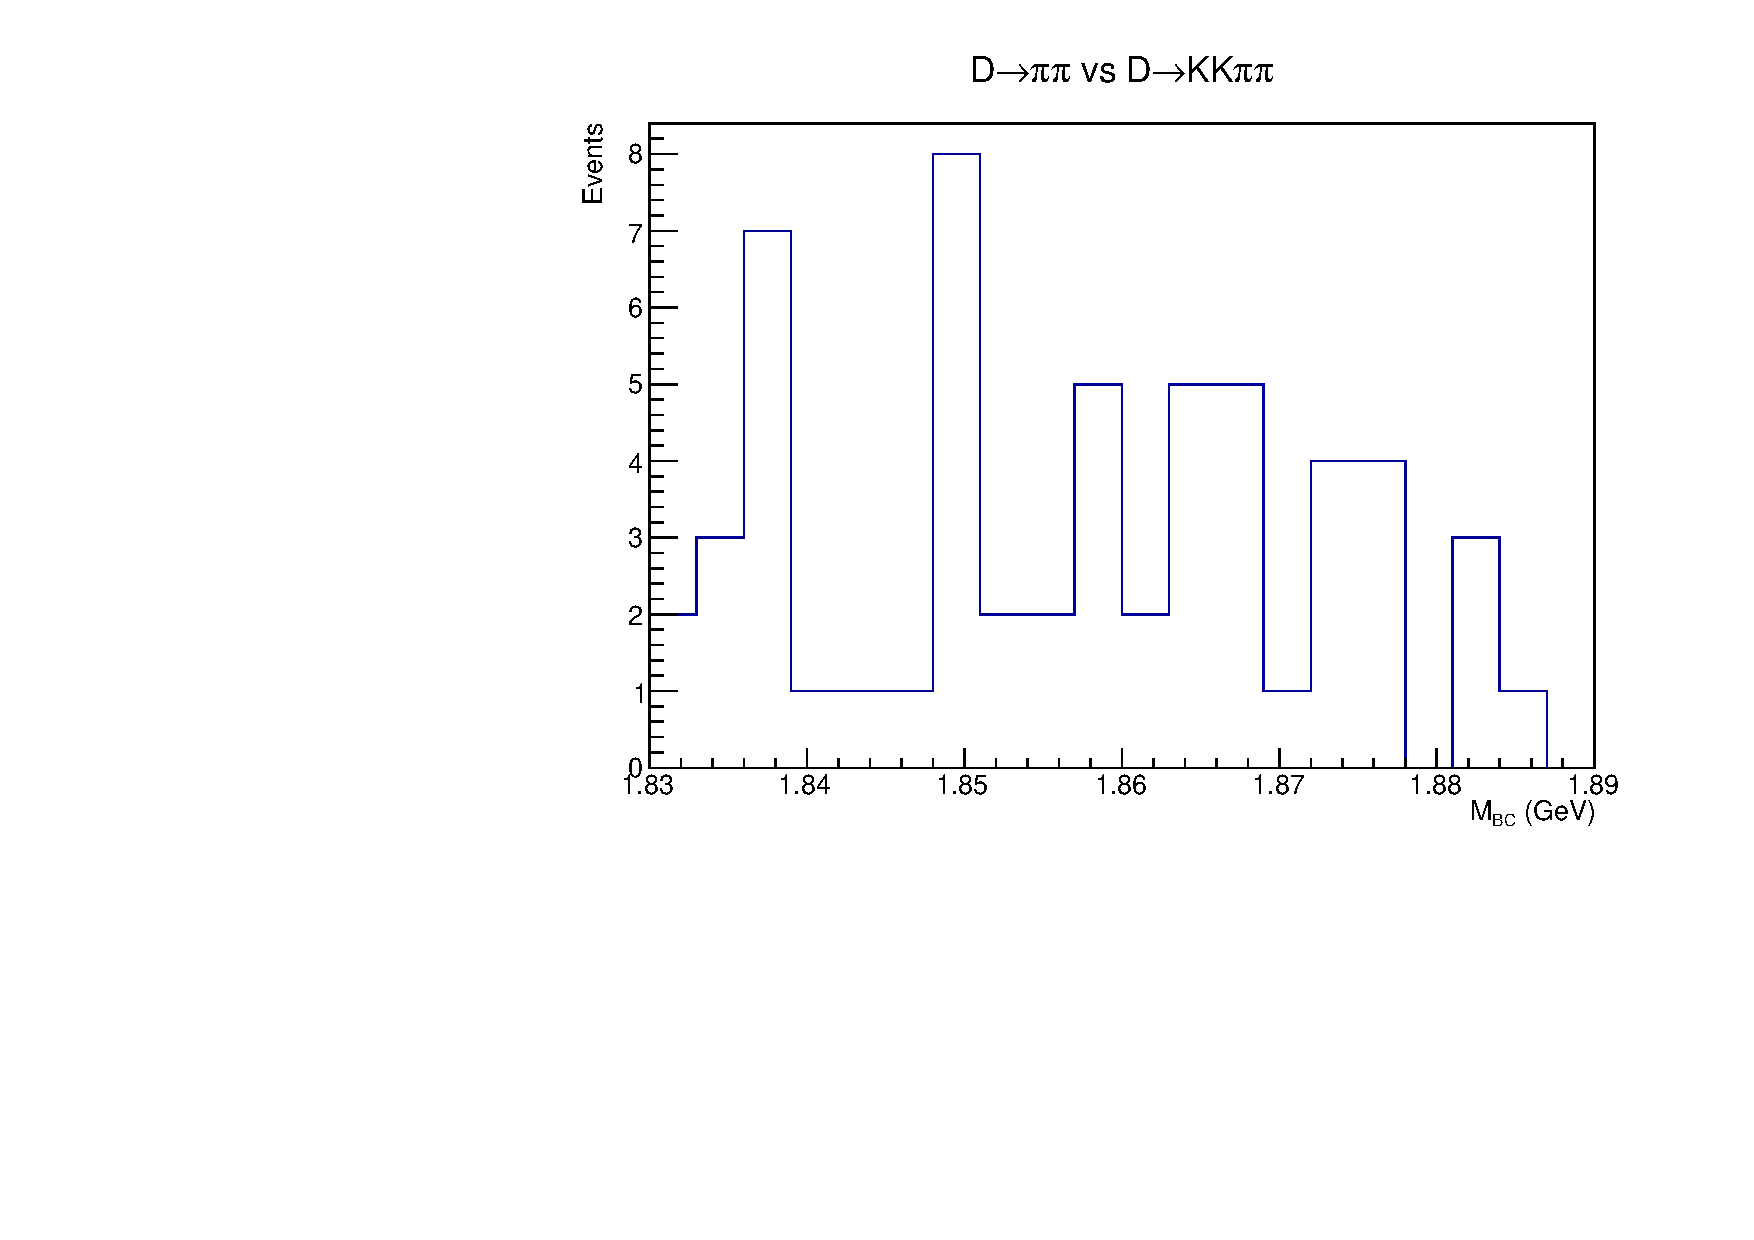
\includegraphics[width = 1.0\textwidth]{Plots/pipi_MBC.pdf}
      \caption{$D\to\pi\pi$ tag}
    \end{subfigure}
    \caption{$D\to KK\pi\pi$ with pionic tags}
  \end{figure}
  \begin{center}
    Flat background mainly from light hadrons, such as $e^+e^-\to K^*\bar{K^*}\rho\to KK\pi\pi\pi\pi$
  \end{center}
\end{frame}

\begin{frame}{Backup: Double tag yields of fully reconstructed events}
  \begin{center}
    However, in the $\pi\pi\pi^0$ tag there is track swap background we can veto\\
    $K\pi\pi^0$ vs $K\pi\pi\pi\rightarrow\pi\pi\pi^0$ vs $KK\pi\pi$\\
    Consider $M_{\rm BC}$ with a track swap:
  \end{center}
  \begin{figure}
    \centering
    \begin{subfigure}{0.4\textwidth}
      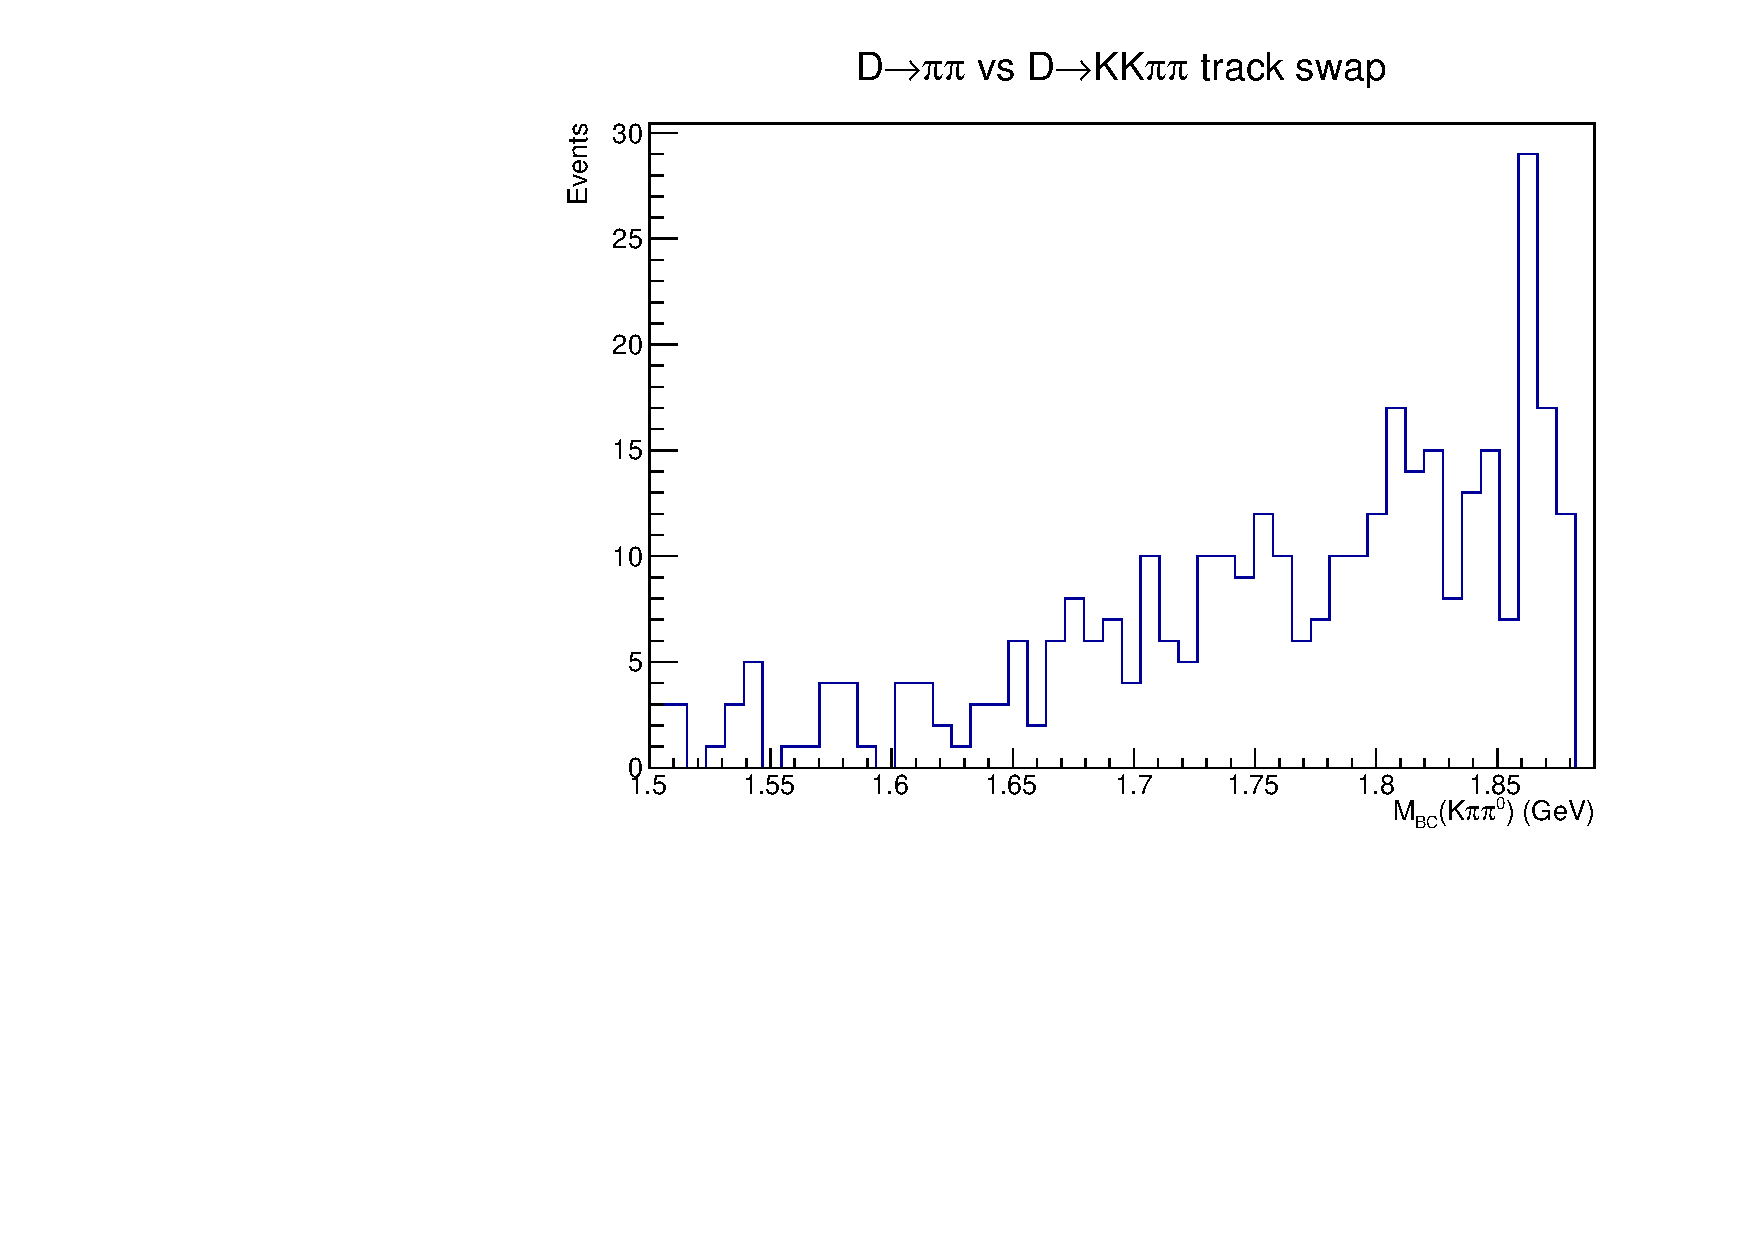
\includegraphics[width = 1.0\textwidth]{Plots/pipipi0_TrackSwap_Kpipi0_MBC.pdf}
      \caption{$D\to K\pi\pi^0$}
    \end{subfigure}%
    \begin{subfigure}{0.4\textwidth}
      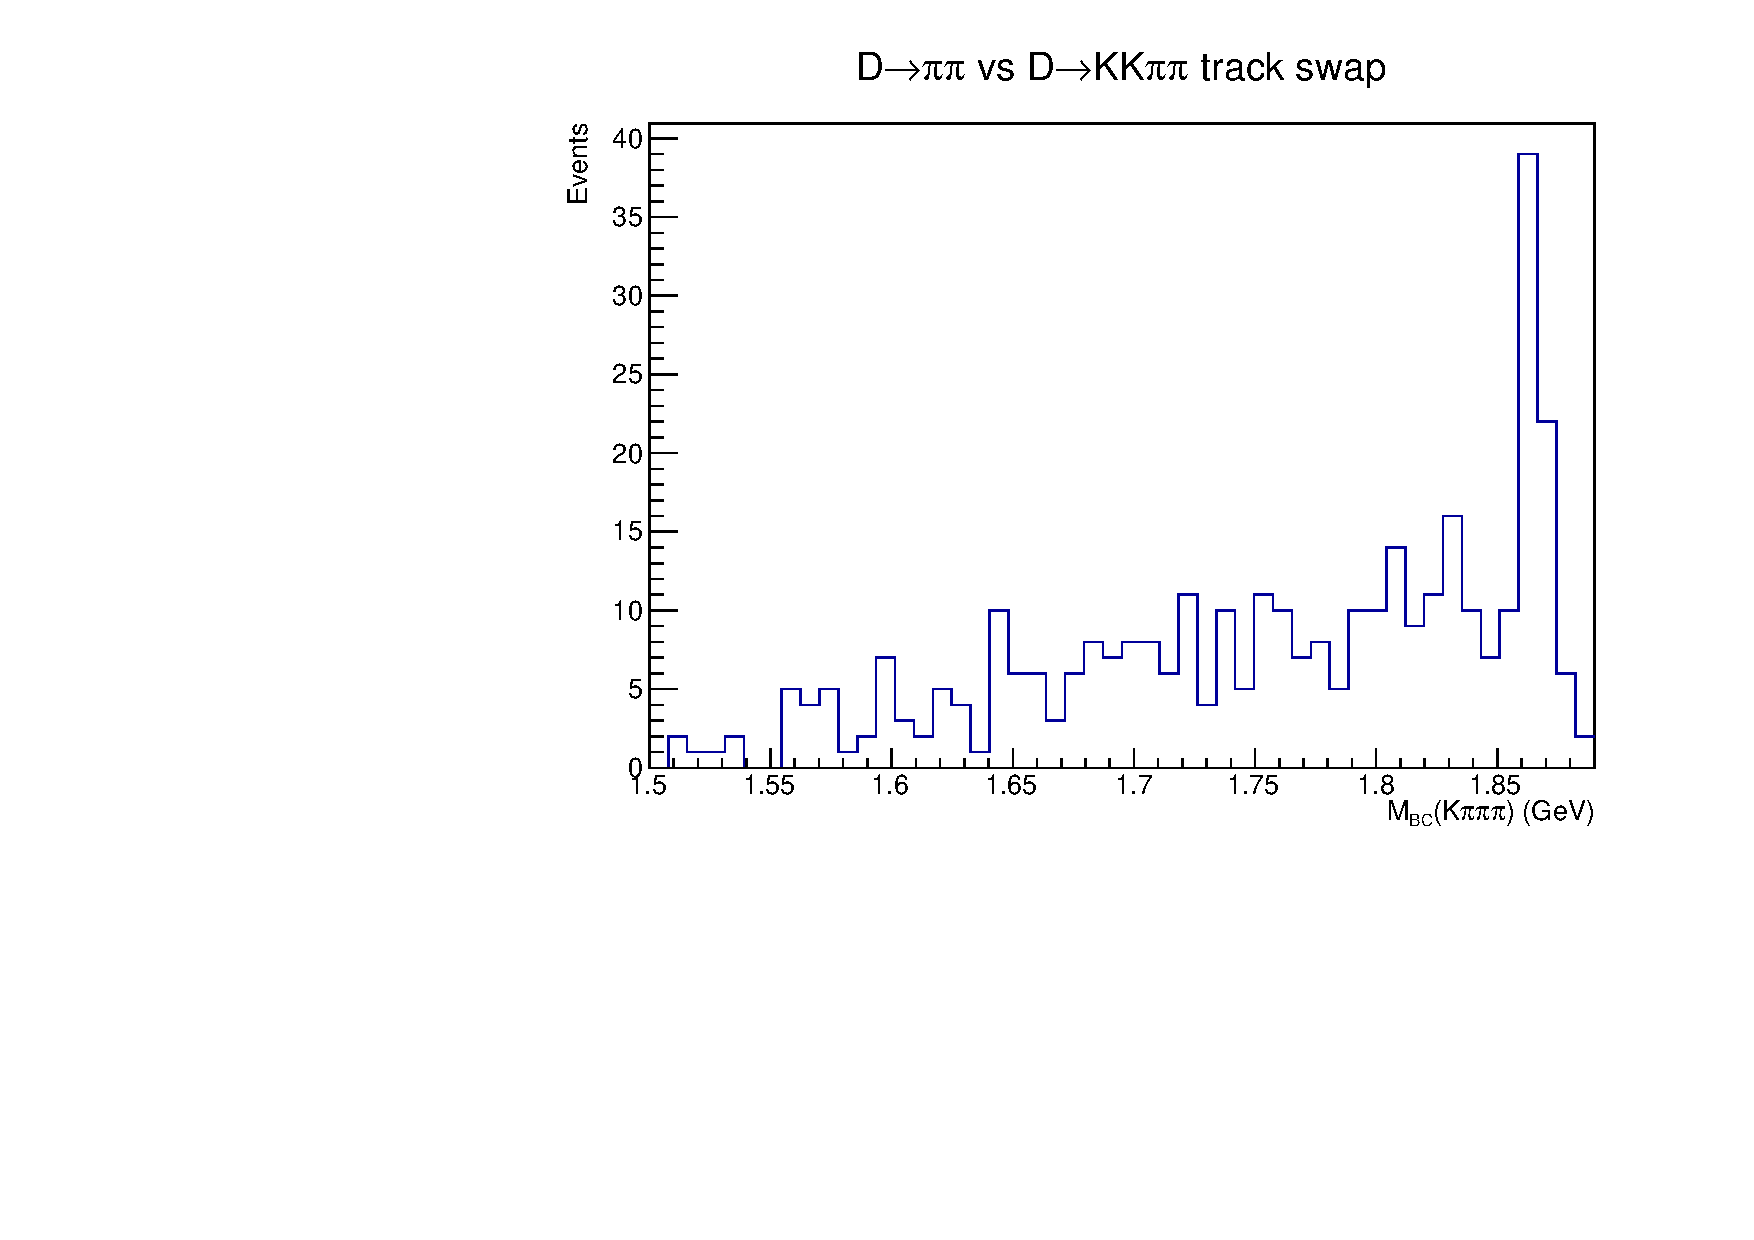
\includegraphics[width = 1.0\textwidth]{Plots/pipipi0_TrackSwap_Kpipipi_MBC.pdf}
      \caption{$D\to K\pi\pi\pi$}
    \end{subfigure}
    \caption{Track swapped $M_{\rm BC}$}
  \end{figure}
  \begin{center}
    A veto in the region $[1.86, 1.87]\si{\giga\eV}$ removes $20\%$ of the flat background
  \end{center}
\end{frame}

\begin{frame}{Backup: Double tag yields of fully reconstructed events}
  \begin{center}
    Double tag yield uncertainties improved, but still lots of background
  \end{center}
  \begin{figure}
    \centering
    \begin{subfigure}{0.4\textwidth}
      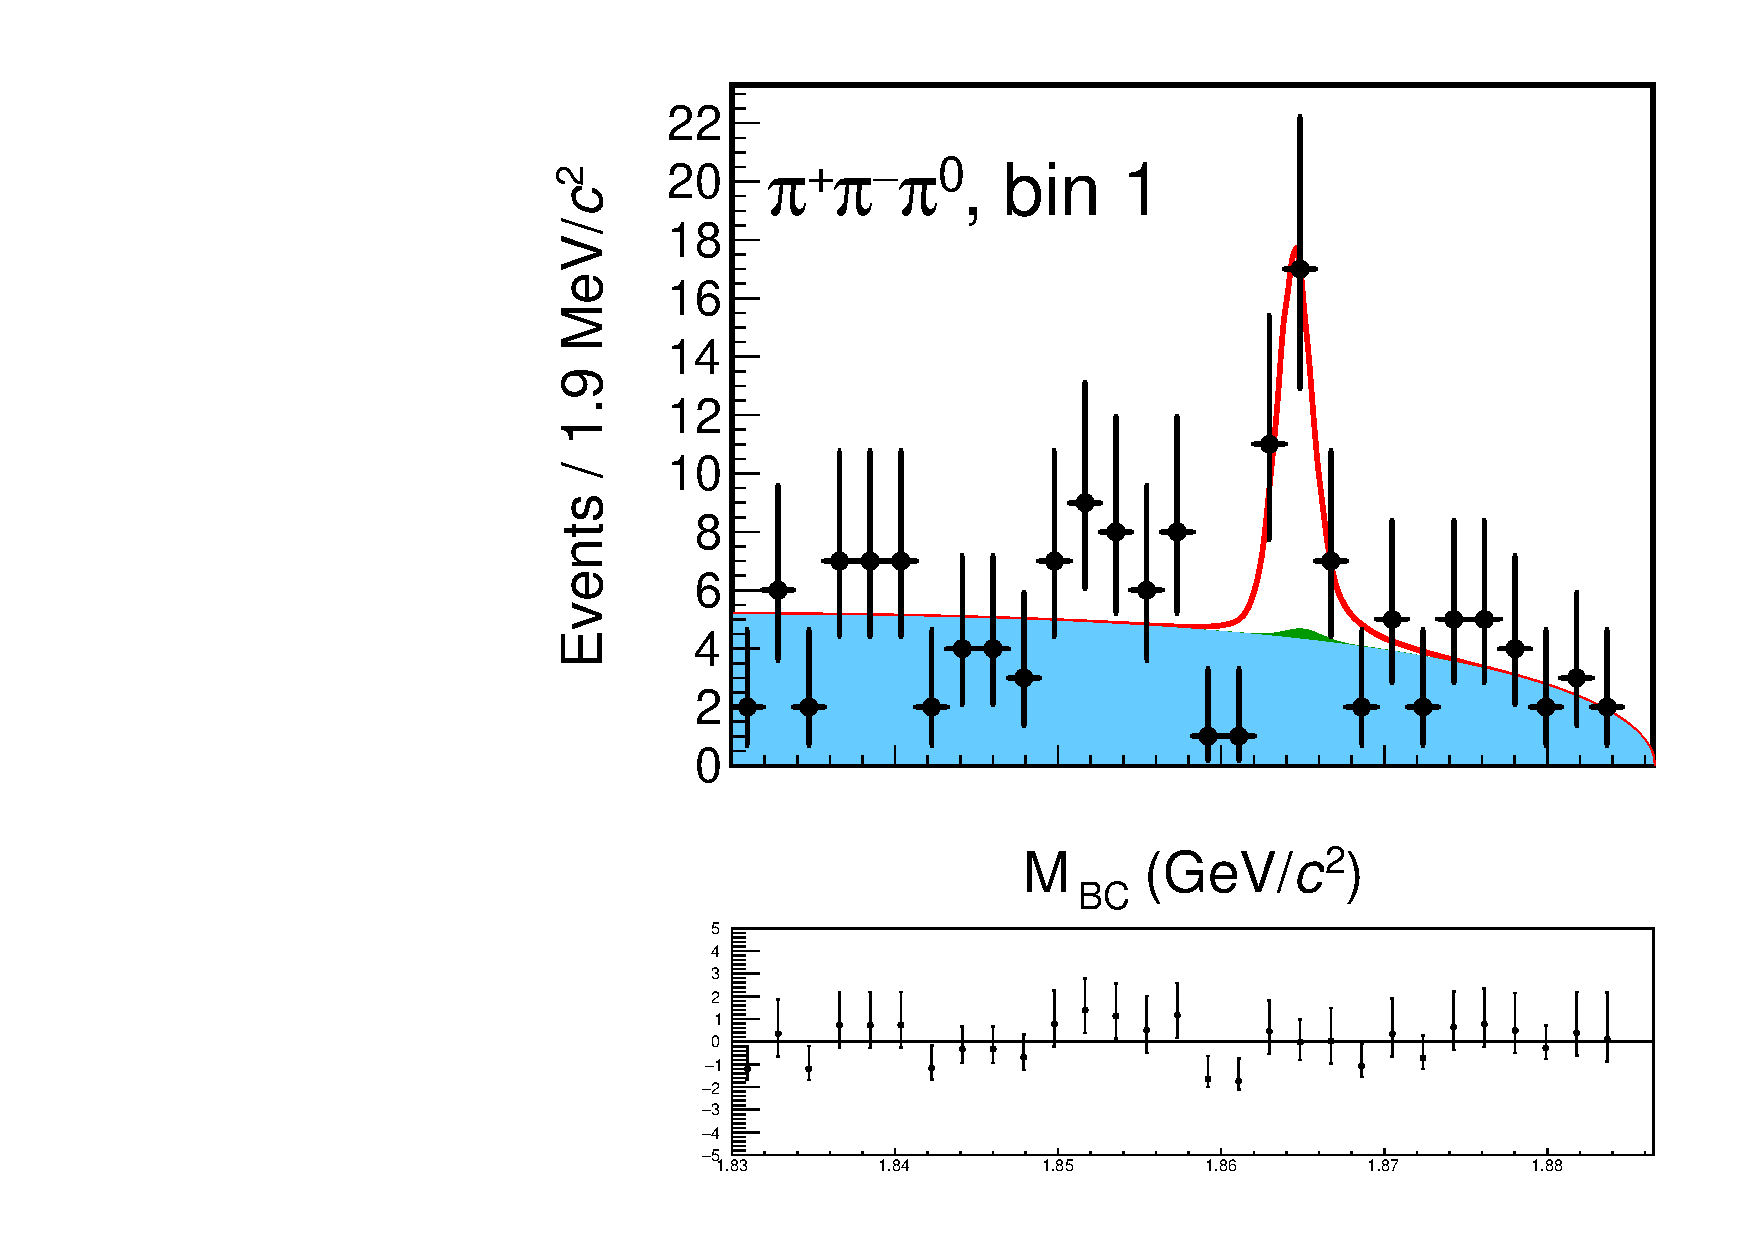
\includegraphics[width = 1.0\textwidth,trim={0 5cm 0 0},clip=true]{Plots/DoubleTagYield_DoubleTag_CP_KKpipi_vs_pipipi0_SignalBin1.pdf}
      \caption{Bin 1, $N^{\rm DT} = 22.6^{+6.4}_{-5.7}$}
    \end{subfigure}%
    \begin{subfigure}{0.4\textwidth}
      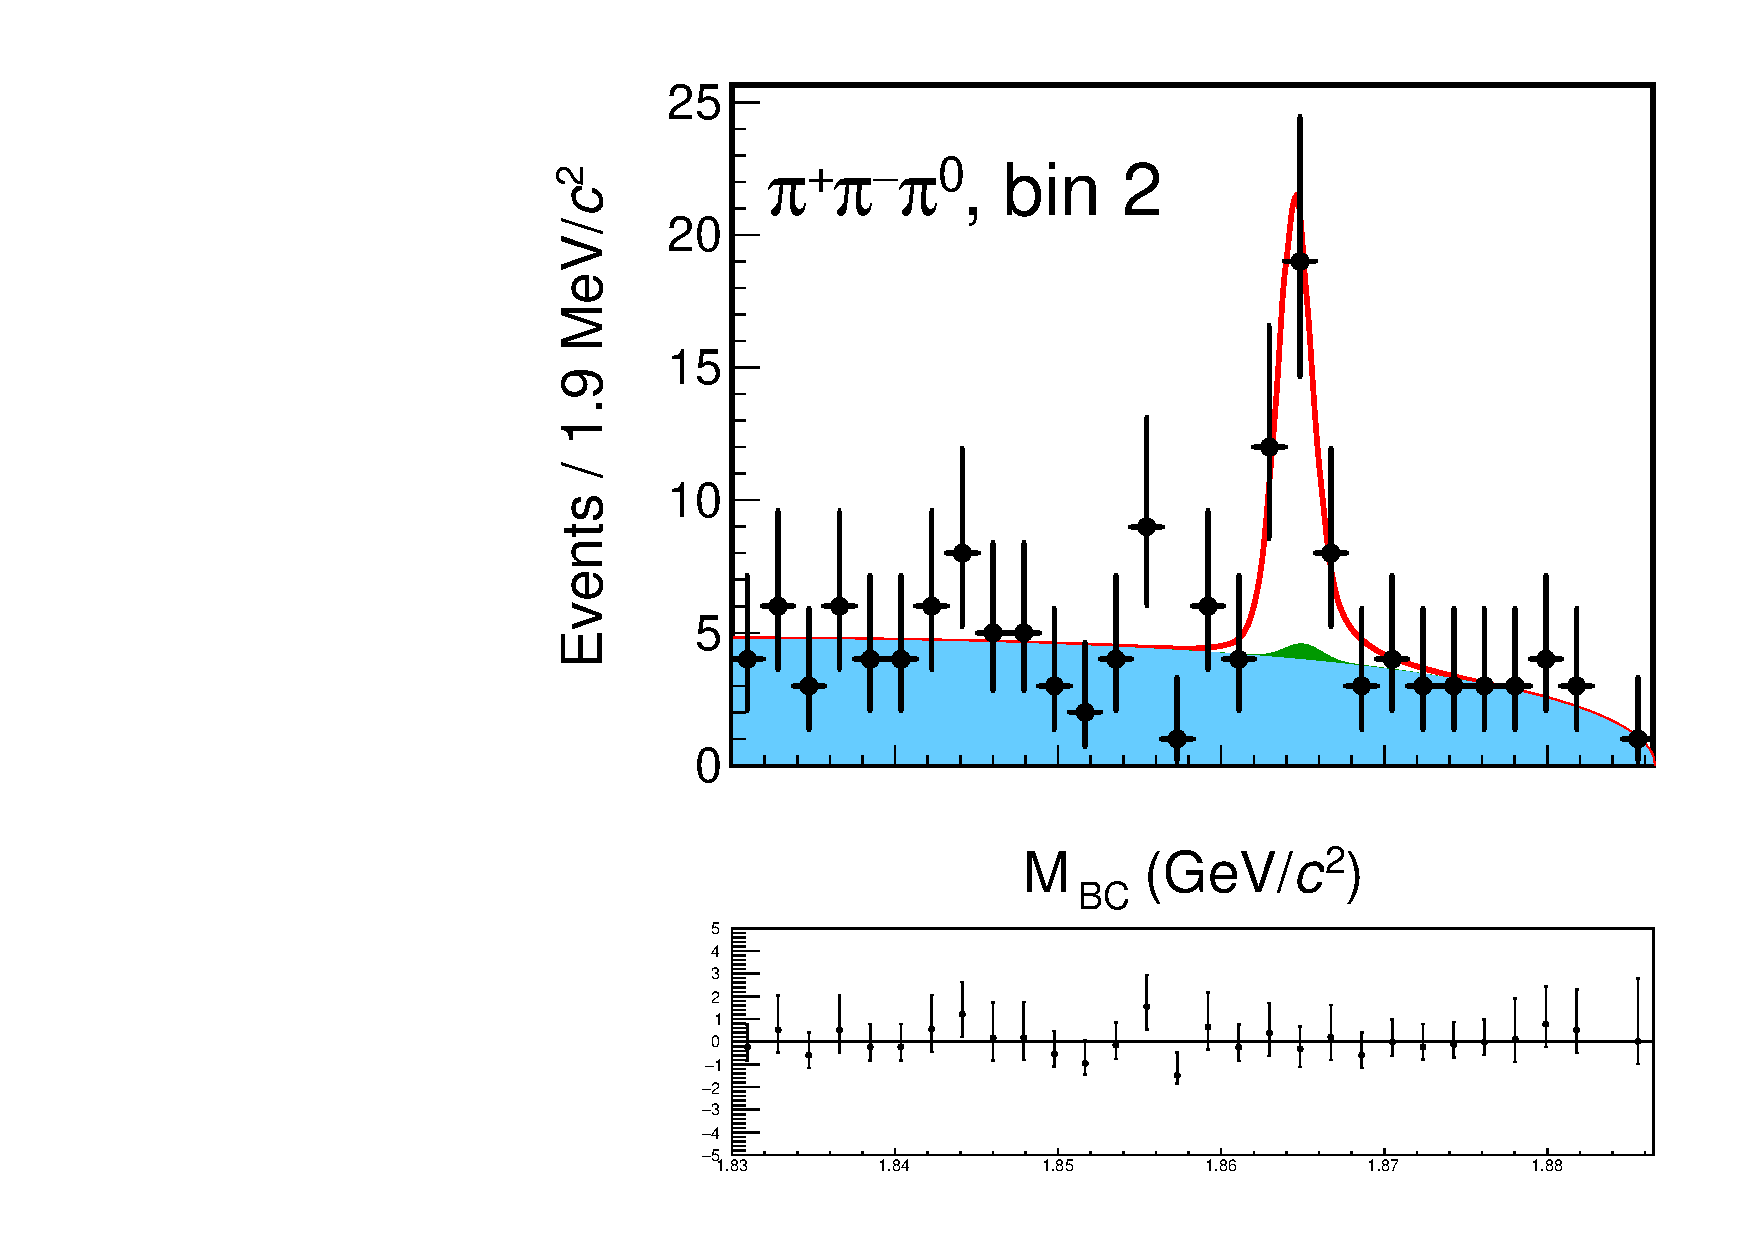
\includegraphics[width = 1.0\textwidth,trim={0 5cm 0 0},clip=true]{Plots/DoubleTagYield_DoubleTag_CP_KKpipi_vs_pipipi0_SignalBin2.pdf}
      \caption{Bin 2, $N^{\rm DT} = 28.1^{+6.9}_{-6.2}$}
    \end{subfigure}
    \caption{Double tag fit of $\pi\pi\pi^0$ tag}
  \end{figure}
\end{frame}

\end{document}